%\documentclass[hyperref={pdfpagelabels=false},slidetop,9pt]{beamer}
\documentclass[slidetop,8pt]{beamer}
\usepackage[T1]{fontenc}
\usepackage[utf8]{inputenc}
\newcommand{\id}{71}
\newcommand{\nom}{Théorie des mécanismes}
\newcommand{\sequence}{04}
\newcommand{\nomsequence}{Liaisons entre les solides}
\newcommand{\num}{02}
\newcommand{\type}{KH}
\newcommand{\descrip}{Liaisons équivalentes, hyperstatisme, liaisons en série et en parallèle, théorie des graphes}
\newcommand{\competences}{B2-12: Proposer une modélisation des liaisons avec leurs caractéristiques géométriques. \\ &  B2-13: Proposer un modèle cinématique paramétré à partir d'un système réel, d'une maquette numérique ou d'u \\ &  B2-17: Simplifier un modèle de mécanisme. \\ &  B2-18: Modifier un modèle pour le rendre isostatique. \\ &  C1-04: Proposer une démarche permettant d'obtenir une loi entrée-sortie géométrique.  \\ &  C2-05: Caractériser le mouvement d'un repère par rapport à un autre repère. \\ &  C2-06: Déterminer les relations entre les grandeurs géométriques ou cinématiques. }
\newcommand{\nbcomp}{7}
\newcommand{\systemes}{}
\newcommand{\systemesnum}{}
\newcommand{\systemessansaccent}{}
\newcommand{\ilot}{2}
\newcommand{\ilotstr}{02}
\newcommand{\dossierilot}{\detokenize{Ilot_02 }}

\usepackage{etex}
\usepackage{tikz}
\usepackage[european]{circuitikz}
\usepackage{pgf}
\usepackage[all]{xy}
\usepackage{pgfpages}
\usepackage{graphbox}
\usepackage{pdfpages}
%\usepackage[adobe-utopia]{mathdesign}
\usepackage{ifthen}
\usepackage{cancel}
\usepackage{framed}
\usepackage{subfig}
\usepackage{tabularx}
\usepackage{setspace}
\usepackage{soul}
\usepackage{schemabloc}
\usepackage{eqnarray}
\usepackage[dot, phantomtext]{dashundergaps}
\usepackage{media9}
\usepackage{multimedia}
\usepackage{textcomp}
\usefonttheme[onlymath]{serif}

\author{Renaud Costadoat}
\institute{Lycée Dorian}

\usepackage{multido}
\usepackage{multirow}
\usepackage{multicol} % Portions de texte en colonnes
\usepackage{flafter}%floatants après la référence

\usepackage{color}
\usepackage{xcolor}
\usepackage{colortbl}

\usepackage[gen]{eurosym}
\usepackage{tikz}
%\usepackage{pstricks,pst-node,pst-tree,pst-solides3d}
\usepackage{lmodern}
\usepackage[francais]{babel}
\usepackage{pslatex}
\usetheme{renaud}
\usepackage{times}
\usepackage[frenchmath]{newtxsf} % for sans serif symbols
\renewcommand{\familydefault}{\sfdefault}
%\usepackage{amsfonts}
%\usepackage{amsmath}
%\usepackage{mathastext}
\usepackage{verbatim}
\usepackage{moreverb}
%\usetikzlibrary{arrows,shapes}
\usepackage{graphicx}
\usepackage{psfrag}
\usepackage{wrapfig}
\usepackage{etoolbox}

\definecolor{gris25}{gray}{0.75}
\definecolor{bleu}{RGB}{18,33,98}
\definecolor{bleuf}{RGB}{42,94,171}
\definecolor{bleuc}{RGB}{231,239,247}
\definecolor{rougef}{RGB}{185,18,27}
\definecolor{rougec}{RGB}{255,188,204}%255,230,231
\definecolor{vertf}{RGB}{103,126,82}
\definecolor{vertc}{RGB}{220,255,191}

\setlength\parindent{24pt}
\parskip 7.2pt
\parindent 8pt

\newenvironment{rem}[1][\hsize]%
{%
    \def\FrameCommand
   {%
\rotatebox{90}{\textit{\textsf{Remarque}}} 
       {\color{bleuf}\vrule width 3pt}%
       \hspace{0pt}%must no space.
       \fboxsep=\FrameSep\colorbox{bleuc}%
  }%
    \MakeFramed{\hsize#1\advance\hsize-\width\FrameRestore}%
}%
{\endMakeFramed}%


\newenvironment{savoir}[1][\hsize]%
{%
    \def\FrameCommand
    {%
\rotatebox{90}{\textit{\textsf{Savoir}}} 
        {\color{bleuf}\vrule width 3pt}%
        \hspace{0pt}%must no space.
        \fboxsep=\FrameSep\colorbox{bleuc}%
    }%
    \MakeFramed{\hsize#1\advance\hsize-\width\FrameRestore}%
}%
{\endMakeFramed}%

\newenvironment{prob}[1][\hsize]%
{%
    \def\FrameCommand%
    {%
\rotatebox{90}{\textit{\textsf{Problematique}}} 
        {\color{rougef}\vrule width 3pt}%
        \hspace{0pt}%must no space.
        \fboxsep=\FrameSep\colorbox{rougec}%
    }%
    \MakeFramed{\hsize#1\advance\hsize-\width\FrameRestore}%
}%
{\endMakeFramed}%

\newenvironment{obj}[1][\hsize]%
{%
    \def\FrameCommand%
    {%
\rotatebox{90}{\textit{\textsf{Objectif}}} 
        {\color{vertf}\vrule width 3pt}%
        \hspace{0pt}%must no space.
        \fboxsep=\FrameSep\colorbox{vertc}%
    }%
    \MakeFramed{\hsize#1\advance\hsize-\width\FrameRestore}%
}%
{\endMakeFramed}%

\newenvironment{defi}[1][\hsize]%
{%
    \def\FrameCommand%
    {%
\rotatebox{90}{\textit{\textsf{Definition}}} 
        {\color{bleuf}\vrule width 3pt}%
        \hspace{0pt}%must no space.
        \fboxsep=\FrameSep\colorbox{rougec}%
    }%
    \MakeFramed{\hsize#1\advance\hsize-\width\FrameRestore}%
}%
{\endMakeFramed}%


\newenvironment{hypo}[1][\hsize]%
{%
    \def\FrameCommand%
    {%
\rotatebox{90}{\textit{\textsf{Hypothèse\\}}} 
        {\color{bleuf}\vrule width 3pt}%
        \hspace{0pt}%must no space.
        \fboxsep=\FrameSep\colorbox{bleuc}%
    }%
    \MakeFramed{\hsize#1\advance\hsize-\width\FrameRestore}%
}%
{\endMakeFramed}%


\newenvironment{prop}[1][\hsize]%
{%
    \def\FrameCommand%
    {%
\rotatebox{90}{\textit{\textsf{Propriété}}} 
        {\color{bleuf}\vrule width 3pt}%
        \hspace{0pt}%must no space.
        \fboxsep=\FrameSep\colorbox{bleuc}%
    }%
    \MakeFramed{\hsize#1\advance\hsize-\width\FrameRestore}%
}%
{\endMakeFramed}%

\newenvironment{props}[1][\hsize]%
{%
    \def\FrameCommand%
    {%
\rotatebox{90}{\textit{\textsf{Propriétés}}} 
        {\color{bleuf}\vrule width 3pt}%
        \hspace{0pt}%must no space.
        \fboxsep=\FrameSep\colorbox{bleuc}%
    }%
    \MakeFramed{\hsize#1\advance\hsize-\width\FrameRestore}%
}%
{\endMakeFramed}%

\newenvironment{exemple}[1][\hsize]%
{%
    \def\FrameCommand%
    {%
\rotatebox{90}{\textit{\textsf{Exemple}}} 
        {\color{vertf}\vrule width 3pt}%
        \hspace{0pt}%must no space.
        \fboxsep=\FrameSep\colorbox{vertc}%
    }%
    \MakeFramed{\hsize#1\advance\hsize-\width\FrameRestore}%
}%
{\endMakeFramed}%

\newenvironment{resultat}[1][\hsize]%
{%
    \def\FrameCommand%
    {%
\rotatebox{90}{\textit{\textsf{Résultat}}} 
        {\color{rougef}\vrule width 3pt}%
%        {\color{bleuf}\vrule width 3pt}%
        \hspace{0pt}%must no space.
        \fboxsep=\FrameSep\colorbox{rougec}%
    }%
    \MakeFramed{\hsize#1\advance\hsize-\width\FrameRestore}%
}%
{\endMakeFramed}%

\newenvironment{methode}[1][\hsize]%
{%
    \def\FrameCommand%
    {%
\rotatebox{90}{\textit{\textsf{Méthode\\}}} 
        {\color{rougef}\vrule width 3pt}%
        \hspace{0pt}%must no space.
        \fboxsep=\FrameSep\colorbox{rougec}%
    }%
    \MakeFramed{\hsize#1\advance\hsize-\width\FrameRestore}%
}%
{\endMakeFramed}%

\newenvironment{theo}[1][\hsize]%
{%
    \def\FrameCommand%
    {%
\rotatebox{90}{\textit{\textsf{Théorème\\}}} 
        {\color{rougef}\vrule width 3pt}%
        \hspace{0pt}%must no space.
        \fboxsep=\FrameSep\colorbox{rougec}%
    }%
    \MakeFramed{\hsize#1\advance\hsize-\width\FrameRestore}%
}%
{\endMakeFramed}%

\newenvironment{warn}[1][\hsize]%
{%
    \def\FrameCommand%
    {%
\rotatebox{90}{\textit{\textsf{Attention\\}}} 
        {\color{rougef}\vrule width 3pt}%
        \hspace{0pt}%must no space.
        \fboxsep=\FrameSep\colorbox{rougec}%
    }%
    \MakeFramed{\hsize#1\advance\hsize-\width\FrameRestore}%
}%
{\endMakeFramed}%

% \usepackage{pstricks}
%\usepackage{minitoc}
% \setcounter{minitocdepth}{4}

\setcounter{tocdepth}{2}

% \mtcselectlanguage{french} 

%\usepackage{draftcopy}% "Brouillon"
% \usepackage{floatflt}
\usepackage{psfrag}
%\usepackage{listings} % Permet d'insérer du code de programmation
\renewcommand{\baselinestretch}{1.2}

% Changer la num�rotation des figures :
% ------------------------------------
% \makeatletter
% \renewcommand{\thefigure}{\ifnum \c@section>\z@ \thesection.\fi
%  \@arabic\c@figure}
% \@addtoreset{figure}{section}
% \makeatother
 


%%%%%%%%%%%%
% Définition des vecteurs %
%%%%%%%%%%%%
 \newcommand{\vect}[1]{\overrightarrow{#1}}

%%%%%%%%%%%%
% Définition des torseusr %
%%%%%%%%%%%%

 \newcommand{\torseur}[1]{%
\left\{{#1}\right\}
}

\newcommand{\torseurcin}[3]{%
\left\{\mathcal{#1} \left(#2/#3 \right) \right\}
}

\newcommand{\torseurstat}[3]{%
\left\{\mathcal{#1} \left(#2\rightarrow #3 \right) \right\}
}

 \newcommand{\torseurc}[8]{%
%\left\{#1 \right\}=
\left\{
{#1}
\right\}
 = 
\left\{%
\begin{array}{cc}%
{#2} & {#5}\\%
{#3} & {#6}\\%
{#4} & {#7}\\%
\end{array}%
\right\}_{#8}%
}

 \newcommand{\torseurcol}[7]{
\left\{%
\begin{array}{cc}%
{#1} & {#4}\\%
{#2} & {#5}\\%
{#3} & {#6}\\%
\end{array}%
\right\}_{#7}%
}

 \newcommand{\torseurl}[3]{%
%\left\{\mathcal{#1}\right\}_{#2}=%
\left\{%
\begin{array}{l}%
{#1} \\%
{#2} %
\end{array}%
\right\}_{#3}%
}

 \newcommand{\vectv}[3]{%
\vect{V\left( {#1} \in {#2}/{#3}\right)}
}


\newcommand{\vectf}[2]{%
\vect{R\left( {#1} \rightarrow {#2}\right)}
}

\newcommand{\vectm}[3]{%
\vect{\mathcal{M}\left( {#1}, {#2} \rightarrow {#3}\right)}
}


 \newcommand{\vectg}[3]{%
\vect{\Gamma \left( {#1} \in {#2}/{#3}\right)}
}

 \newcommand{\vecto}[2]{%
\vect{\Omega\left( {#1}/{#2}\right)}
}

\newcommand{\reponse}[1][4]
{
\multido{}{#1}
{
\begin{center}
\makebox[0.9\linewidth]{\dotfill} \end{center}
}}


% }$$\left\{\mathcal{#1} \right\}_{#2} =%
% \left\{%
% \begin{array}{c}%
%  #3 \\%
%  #4 %
% \end{array}%
% \right\}_{#5}}


%  ------------------------------------------
% | Modification du formatage des sections : | 
%  ------------------------------------------

% Grands titres :
% ---------------

\newcommand{\titre}[1]{%
\begin{center}
      \bigskip
      \rule{\textwidth}{1pt}
      \par\vspace{0.1cm}
      
      \textbf{\large #1}
      \par\rule{\textwidth}{1pt}
    \end{center}
    \bigskip
  }

% Supprime le numéro du chapitre dans la numérotation des sections:
% -----------------------------------------------------------------
\makeatletter
\renewcommand{\thesection}{\@arabic\c@section}
\makeatother


% \titleformat{\chapter}[display]
% {\normalfont\Large\filcenter}
% {}
% {1pc}
% {\titlerule[1pt]
%   \vspace{1pc}%
%   \Huge}[\vspace{1ex}%
% \titlerule]


%%%% Chapitres Comme PY Pechard %%%%%%%%%
% numéro du chapitre
\DeclareFixedFont{\chapnumfont}{OT1}{phv}{b}{n}{80pt}
% pour le mot " Chapitre "
\DeclareFixedFont{\chapchapfont}{OT1}{phv}{m}{it}{40pt}
% pour le titre
\DeclareFixedFont{\chaptitfont}{T1}{phv}{b}{n}{25pt}

\definecolor{gris}{gray}{0.75}
\setbeamertemplate{section in toc}[sections numbered]

\newlength{\RoundedBoxWidth}
\newsavebox{\GrayRoundedBox}
\newenvironment{GrayBox}[1][\dimexpr\textwidth-4.5ex]%
   {\setlength{\RoundedBoxWidth}{\dimexpr#1}
    \begin{lrbox}{\GrayRoundedBox}
       \begin{minipage}{\RoundedBoxWidth}}%
   {   \end{minipage}
    \end{lrbox}
    \begin{center}
    \begin{tikzpicture}%
       \draw node[draw=bleuf,fill=bleuc,rounded corners,%
             inner sep=2ex,text width=\RoundedBoxWidth]%
             {\usebox{\GrayRoundedBox}};
    \end{tikzpicture}
    \end{center}}
    
\ifdef{\prive}{\pgfpagesuselayout{2 on 1}[a4paper,border shrink=0mm]}
\ifdef{\prive}{\setbeamertemplate{navigation symbols}{}}
\setbeamertemplate{itemize item}[ball]
%\setbeamertemplate{blocks}[rounded]%[shadow=true]
\setbeamercolor{block title}{fg=white,bg=grisf}        % titre block normal 
\setbeamercolor{block body}{fg=grisf,bg=grisc!50}      % corps block normal
\setbeamercolor{block body alerted}{fg=white,bg=warning}   % idem pour un block alerte

\title{\nom}
\date{S\sequence \ - \type\num}

\begin{document}
\shorthandoff{:!}
\bibliographystyle{abbrvnat-fr}

\usebackgroundtemplate%
{%
    \centering
\includegraphics[width=\paperwidth]{/home/renaud/Documents/Renaud/GitHub/Sciences-Ingenieur/img/fond2}%
}

{
\setbeamertemplate{navigation symbols}{}
\setbeamertemplate{headline}[pagetitre]
\setbeamertemplate{footline}[pagetitre]
\usebackgroundtemplate{\centering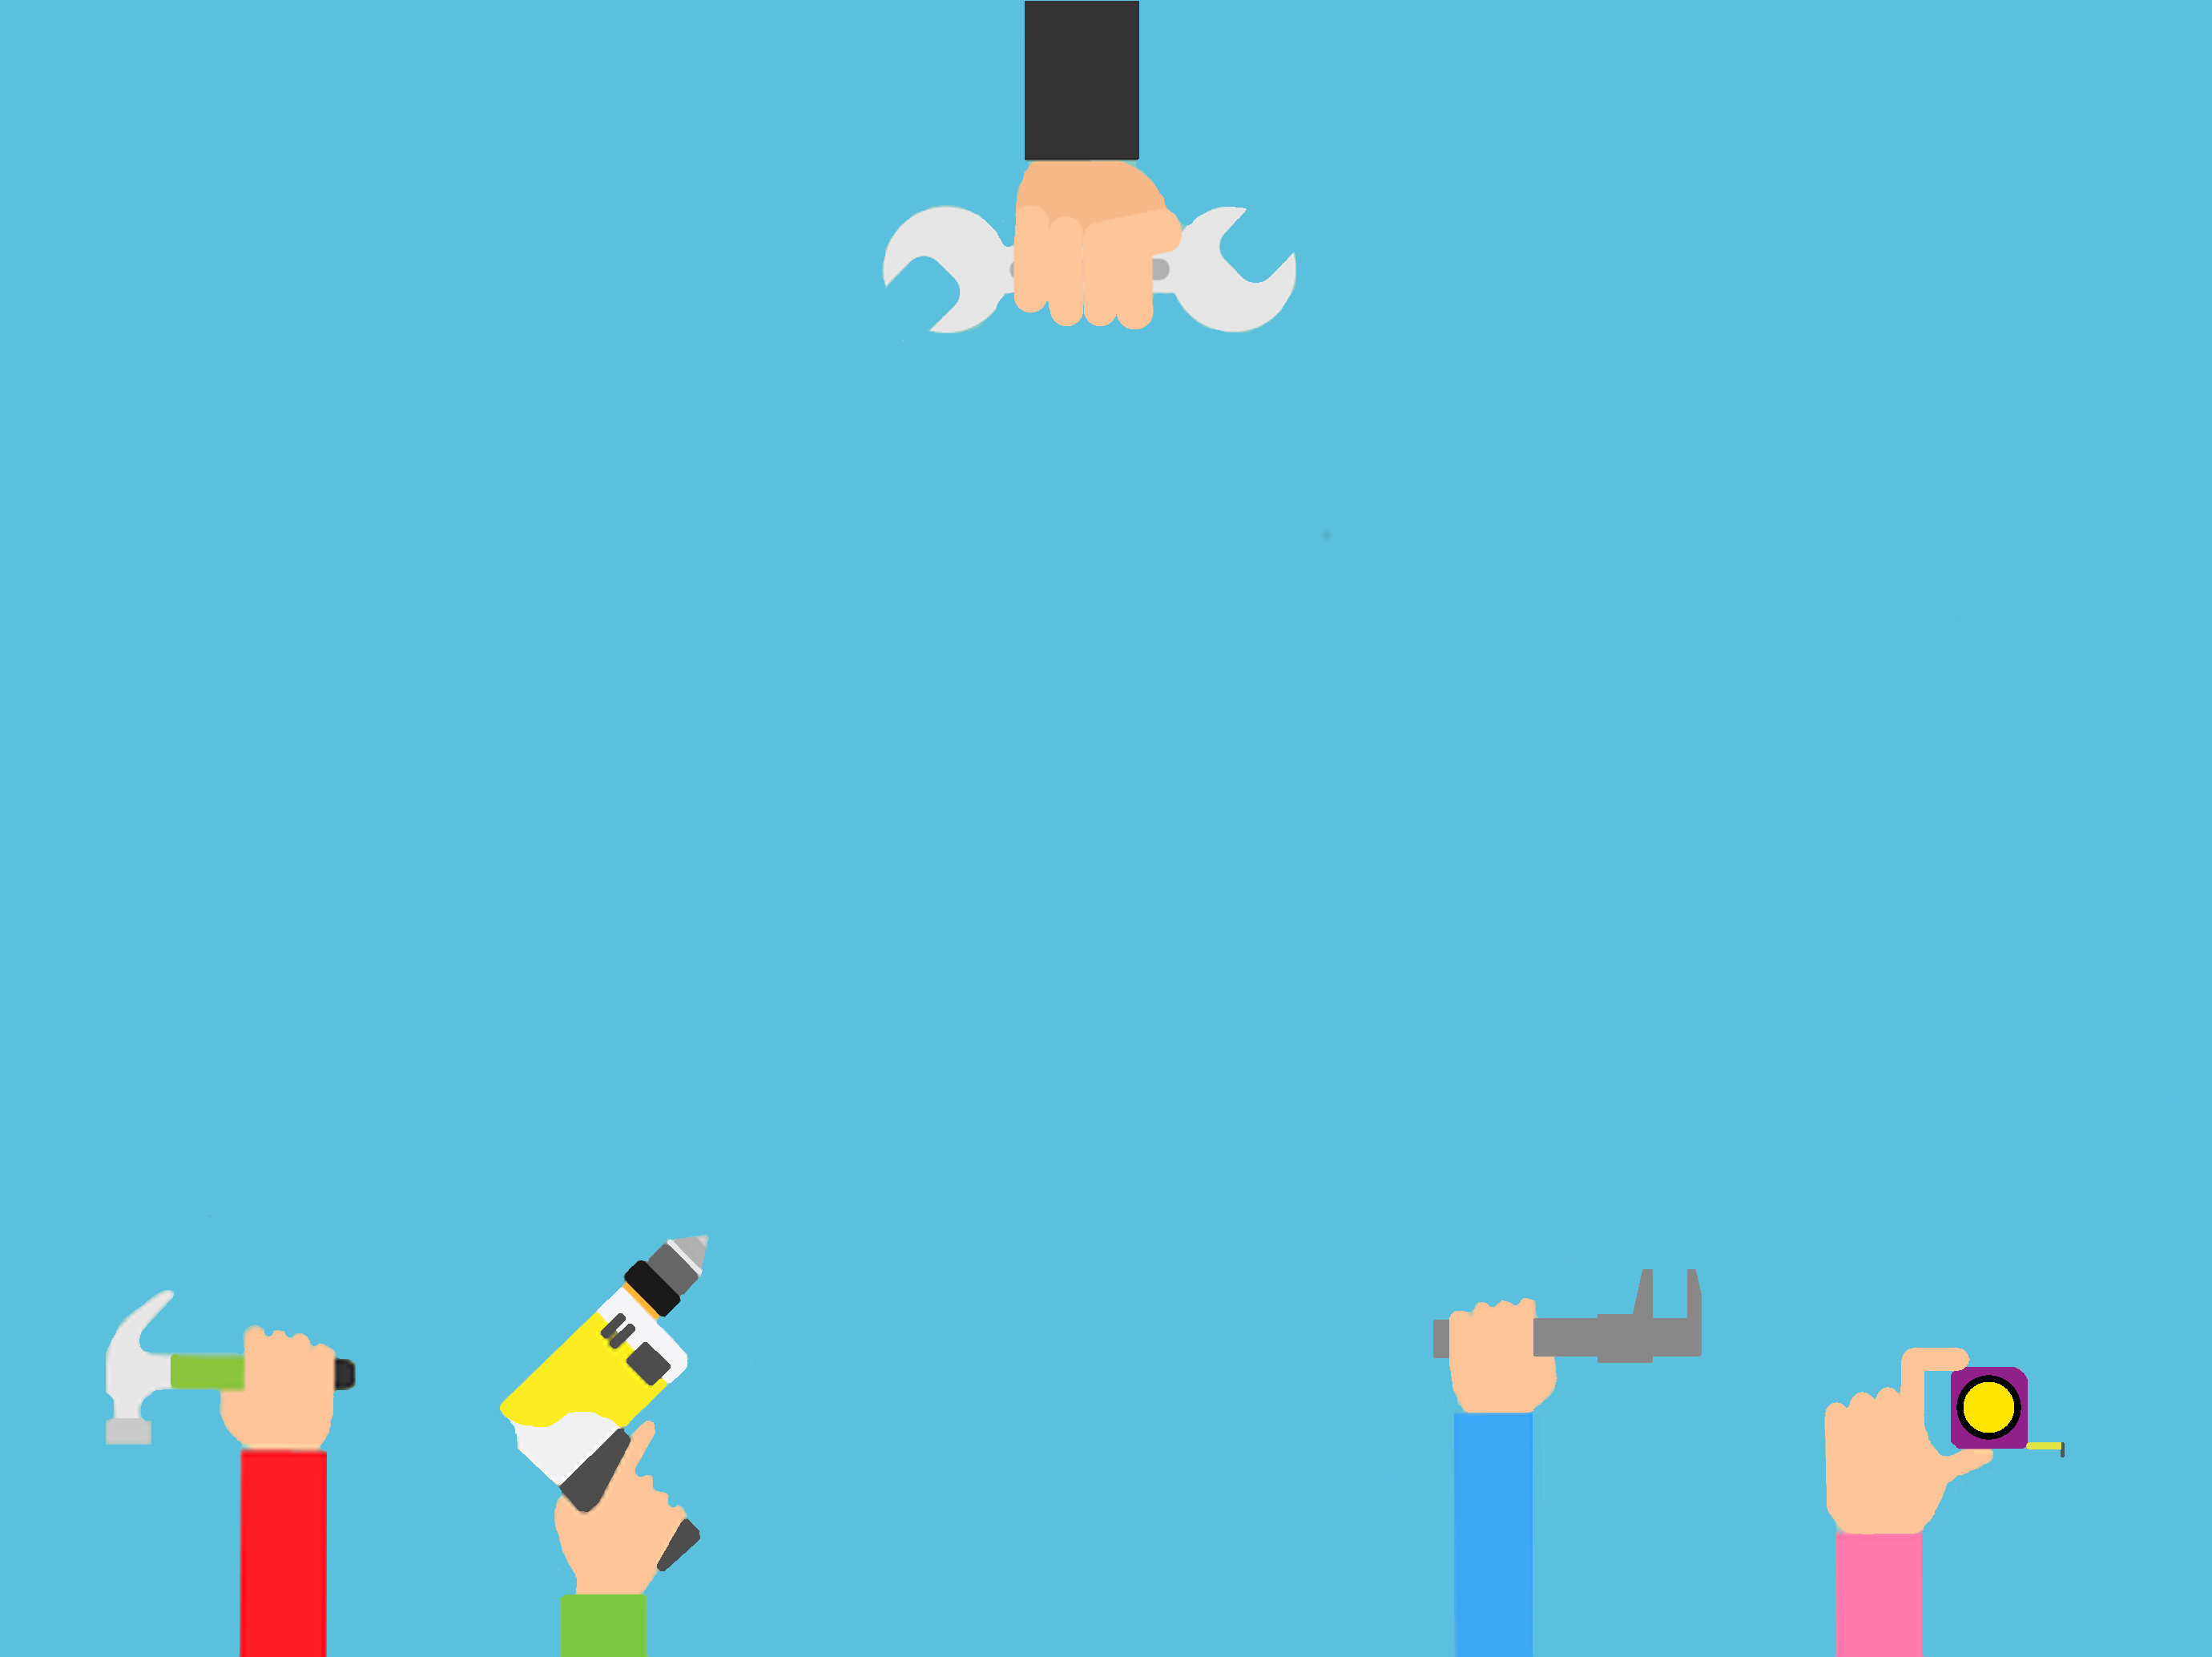
\includegraphics[width=\paperwidth]{/home/renaud/Documents/Renaud/GitHub/Sciences-Ingenieur/img/fond}}
\frame{\titlepage}
}



\section{La chaîne d'énergie}


{\frame{
\frametitle{La décomposition d'un système}


\begin{savoir}

Vous devez être capables de décomposer un produit ou un système.

\begin{itemize}
 \item Quelles sont les composants de ce système ?
 \item Quels sont les liens qui les relient ?
 \item Quels flux circulent entre eux ?
\end{itemize}
\end{savoir}

\begin{prob}

Deux systèmes qui peuvent paraître très différents au départ peuvent avoir des points communs dans leur structure.
\begin{itemize}
 \item \textit{Problème: Comment regrouper les composants d'un système par leur fonction?}
 \item \textbf{Perspectives}: Appliquer une structure de base à tout système afin de déterminer la fonction de ses composants.
\end{itemize}
\end{prob}
}}

{\frame{
\frametitle{Les chaînes d'énergie et d'information}

Sur un \textbf{système complexe}, il est souvent nécessaire de \textbf{décomposer} son étude en plusieurs parties. Il existe plusieurs possibilités pour effectuer cette décomposition, celle qui va être vue maintenant revient à effectuer une isolation des \textbf{chaînes fonctionnelles}.

\ifdef{\public}{\begin{center}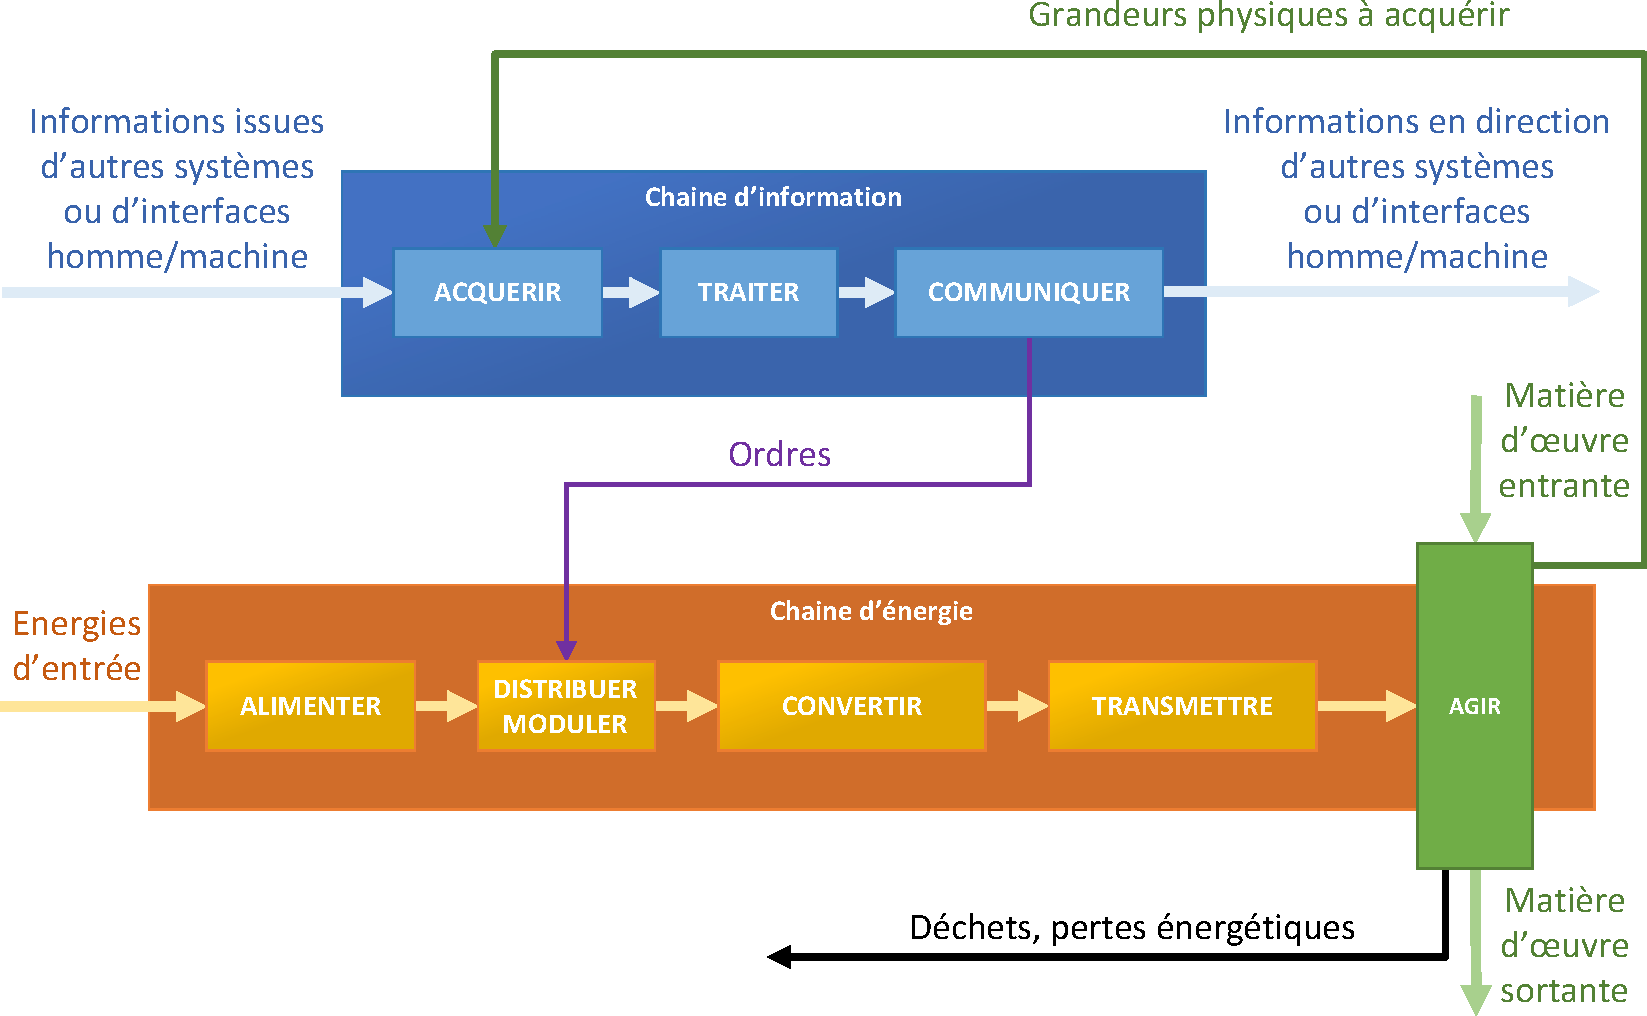
\includegraphics[width=0.8\linewidth]{img/Chaines}\end{center}}
{\begin{center}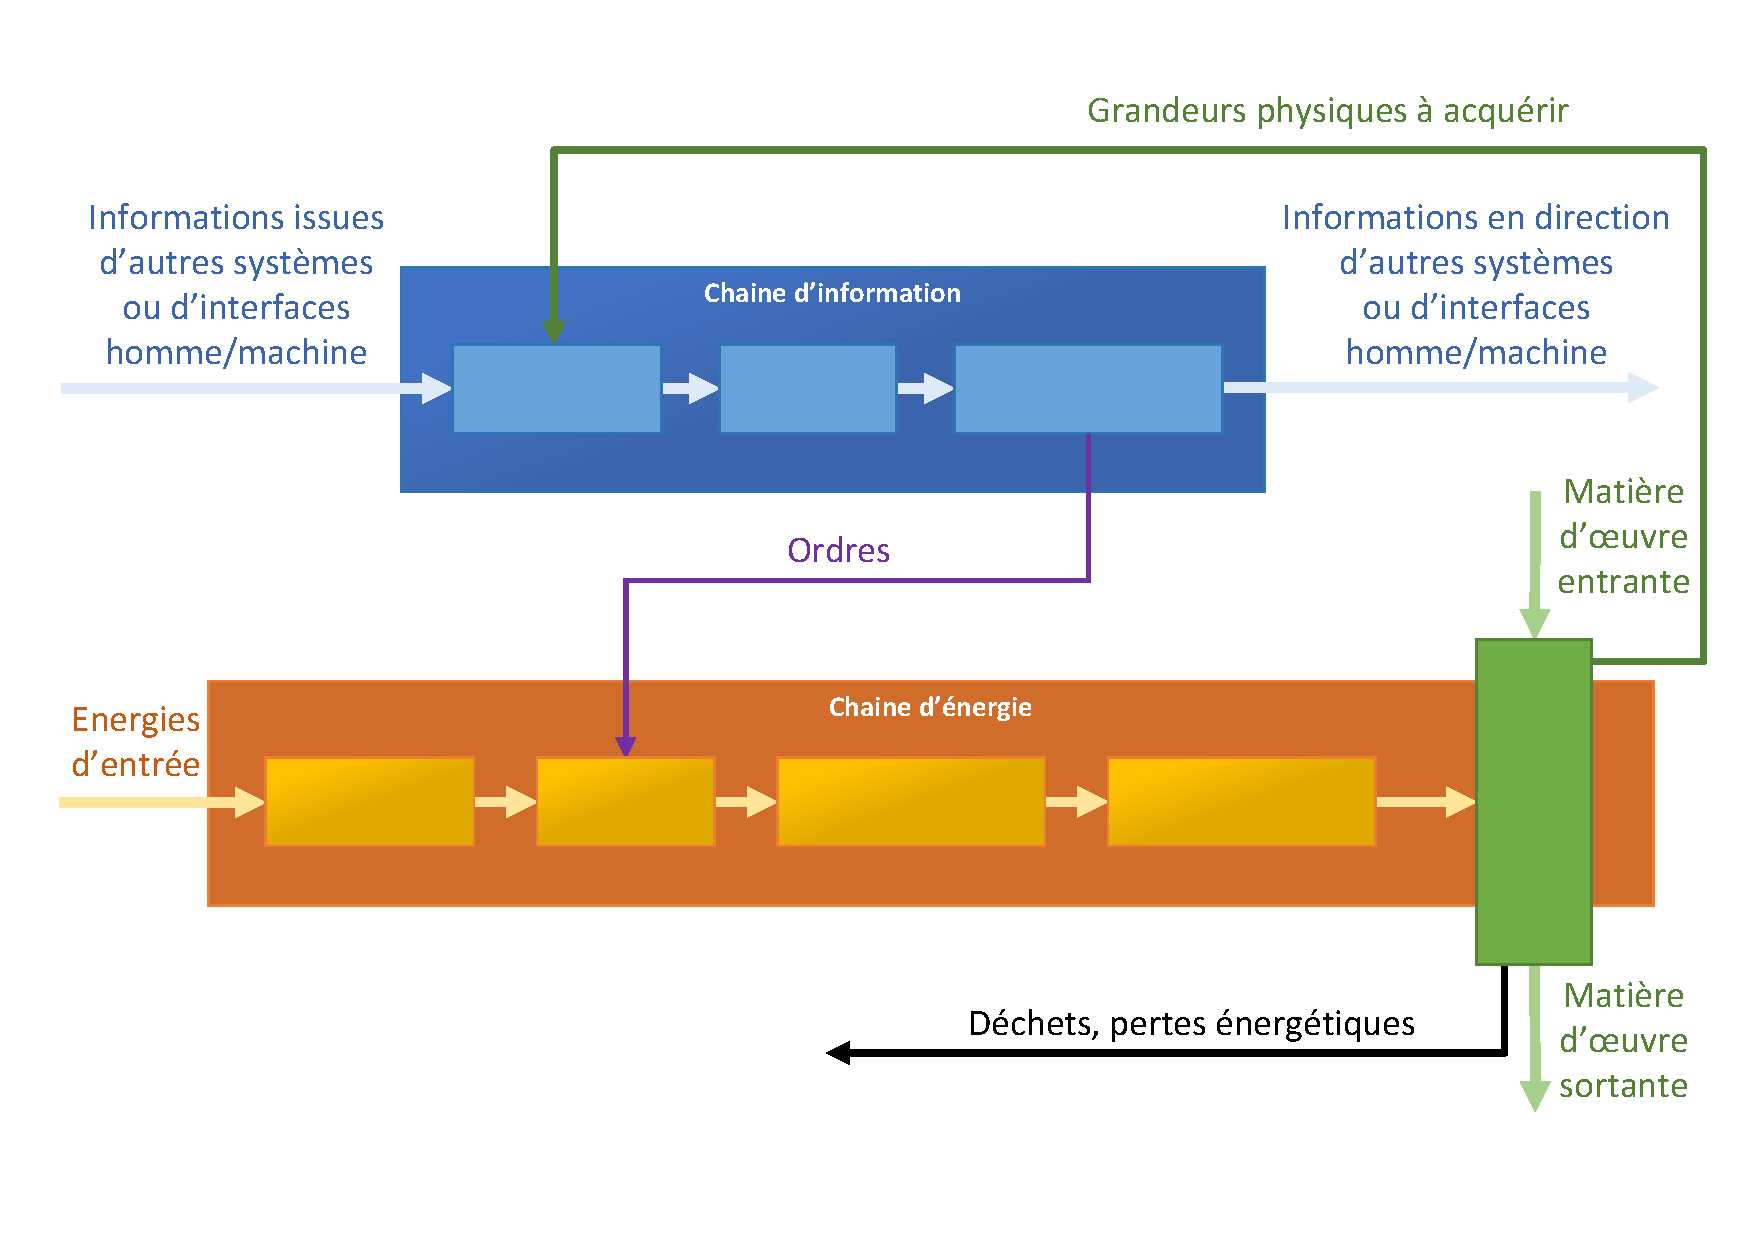
\includegraphics[width=0.8\linewidth]{img/Chaines_vide}\end{center}}
}}

\ifdef{\public}{\begin{frame}
\frametitle{Table des matières}
\tableofcontents[currentsection]
\end{frame}}

{\frame{
\frametitle{La chaîne d'énergie}

C'est par la \textbf{chaîne d'énergie} que transite la \textbf{puissance} nécessaire au système pour fonctionner.

\ifdef{\public}{\begin{center}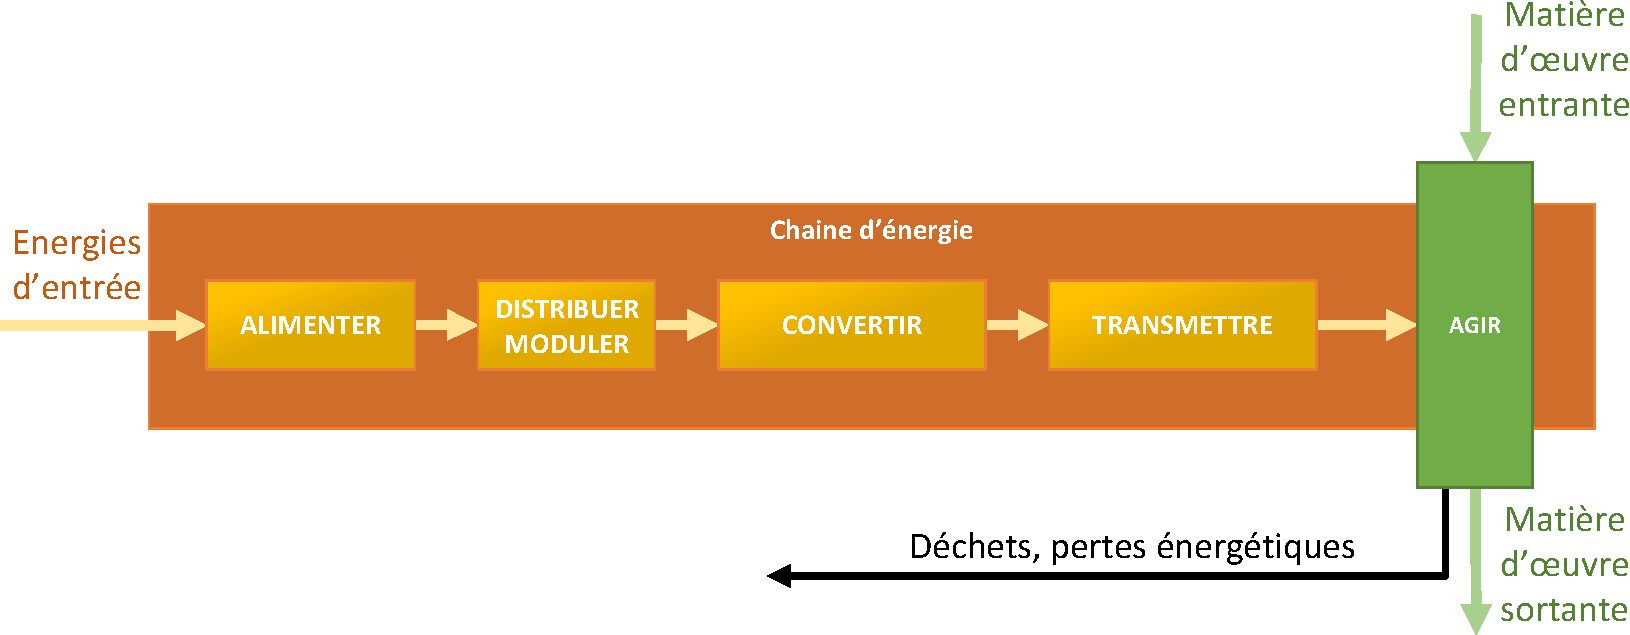
\includegraphics[width=0.8\linewidth]{img/Chaine_energie}\end{center}}
{\begin{center}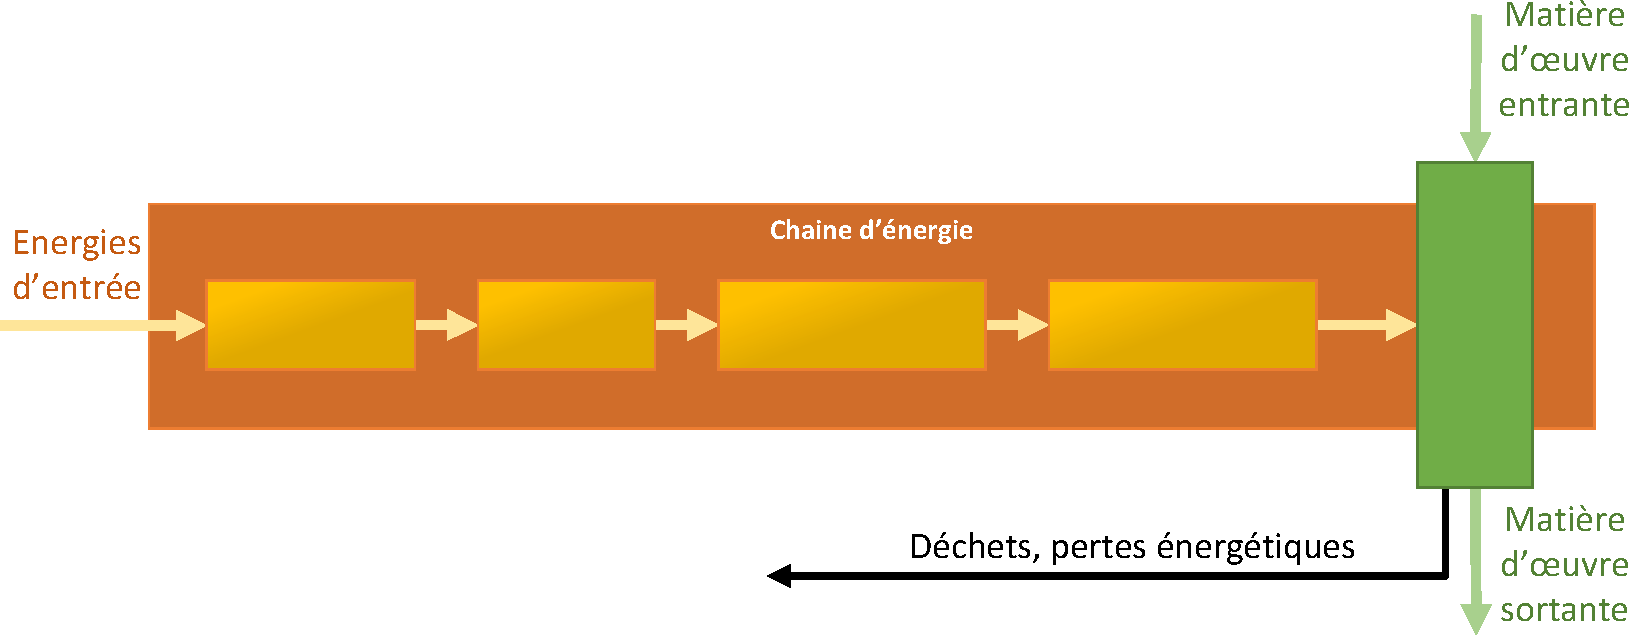
\includegraphics[width=0.8\linewidth]{img/Chaine_energie_vide}\end{center}}


Nous allons détailler les fonctions de cette chaîne:
\begin{itemize}
 \item Alimenter,
 \item Distribuer/moduler,
 \item Convertir,
 \item Transmettre. 
\end{itemize}
}}

{\frame{
\frametitle{Alimenter}

La fonction \textbf{Alimenter} consiste à fournir au système l'énergie qui lui est nécessaire.


\begin{center}
\begin{tabular}{|c|c|c|c|}
\hline
Pile électrique & Réseau électrique & Eolien & Solaire \\ 
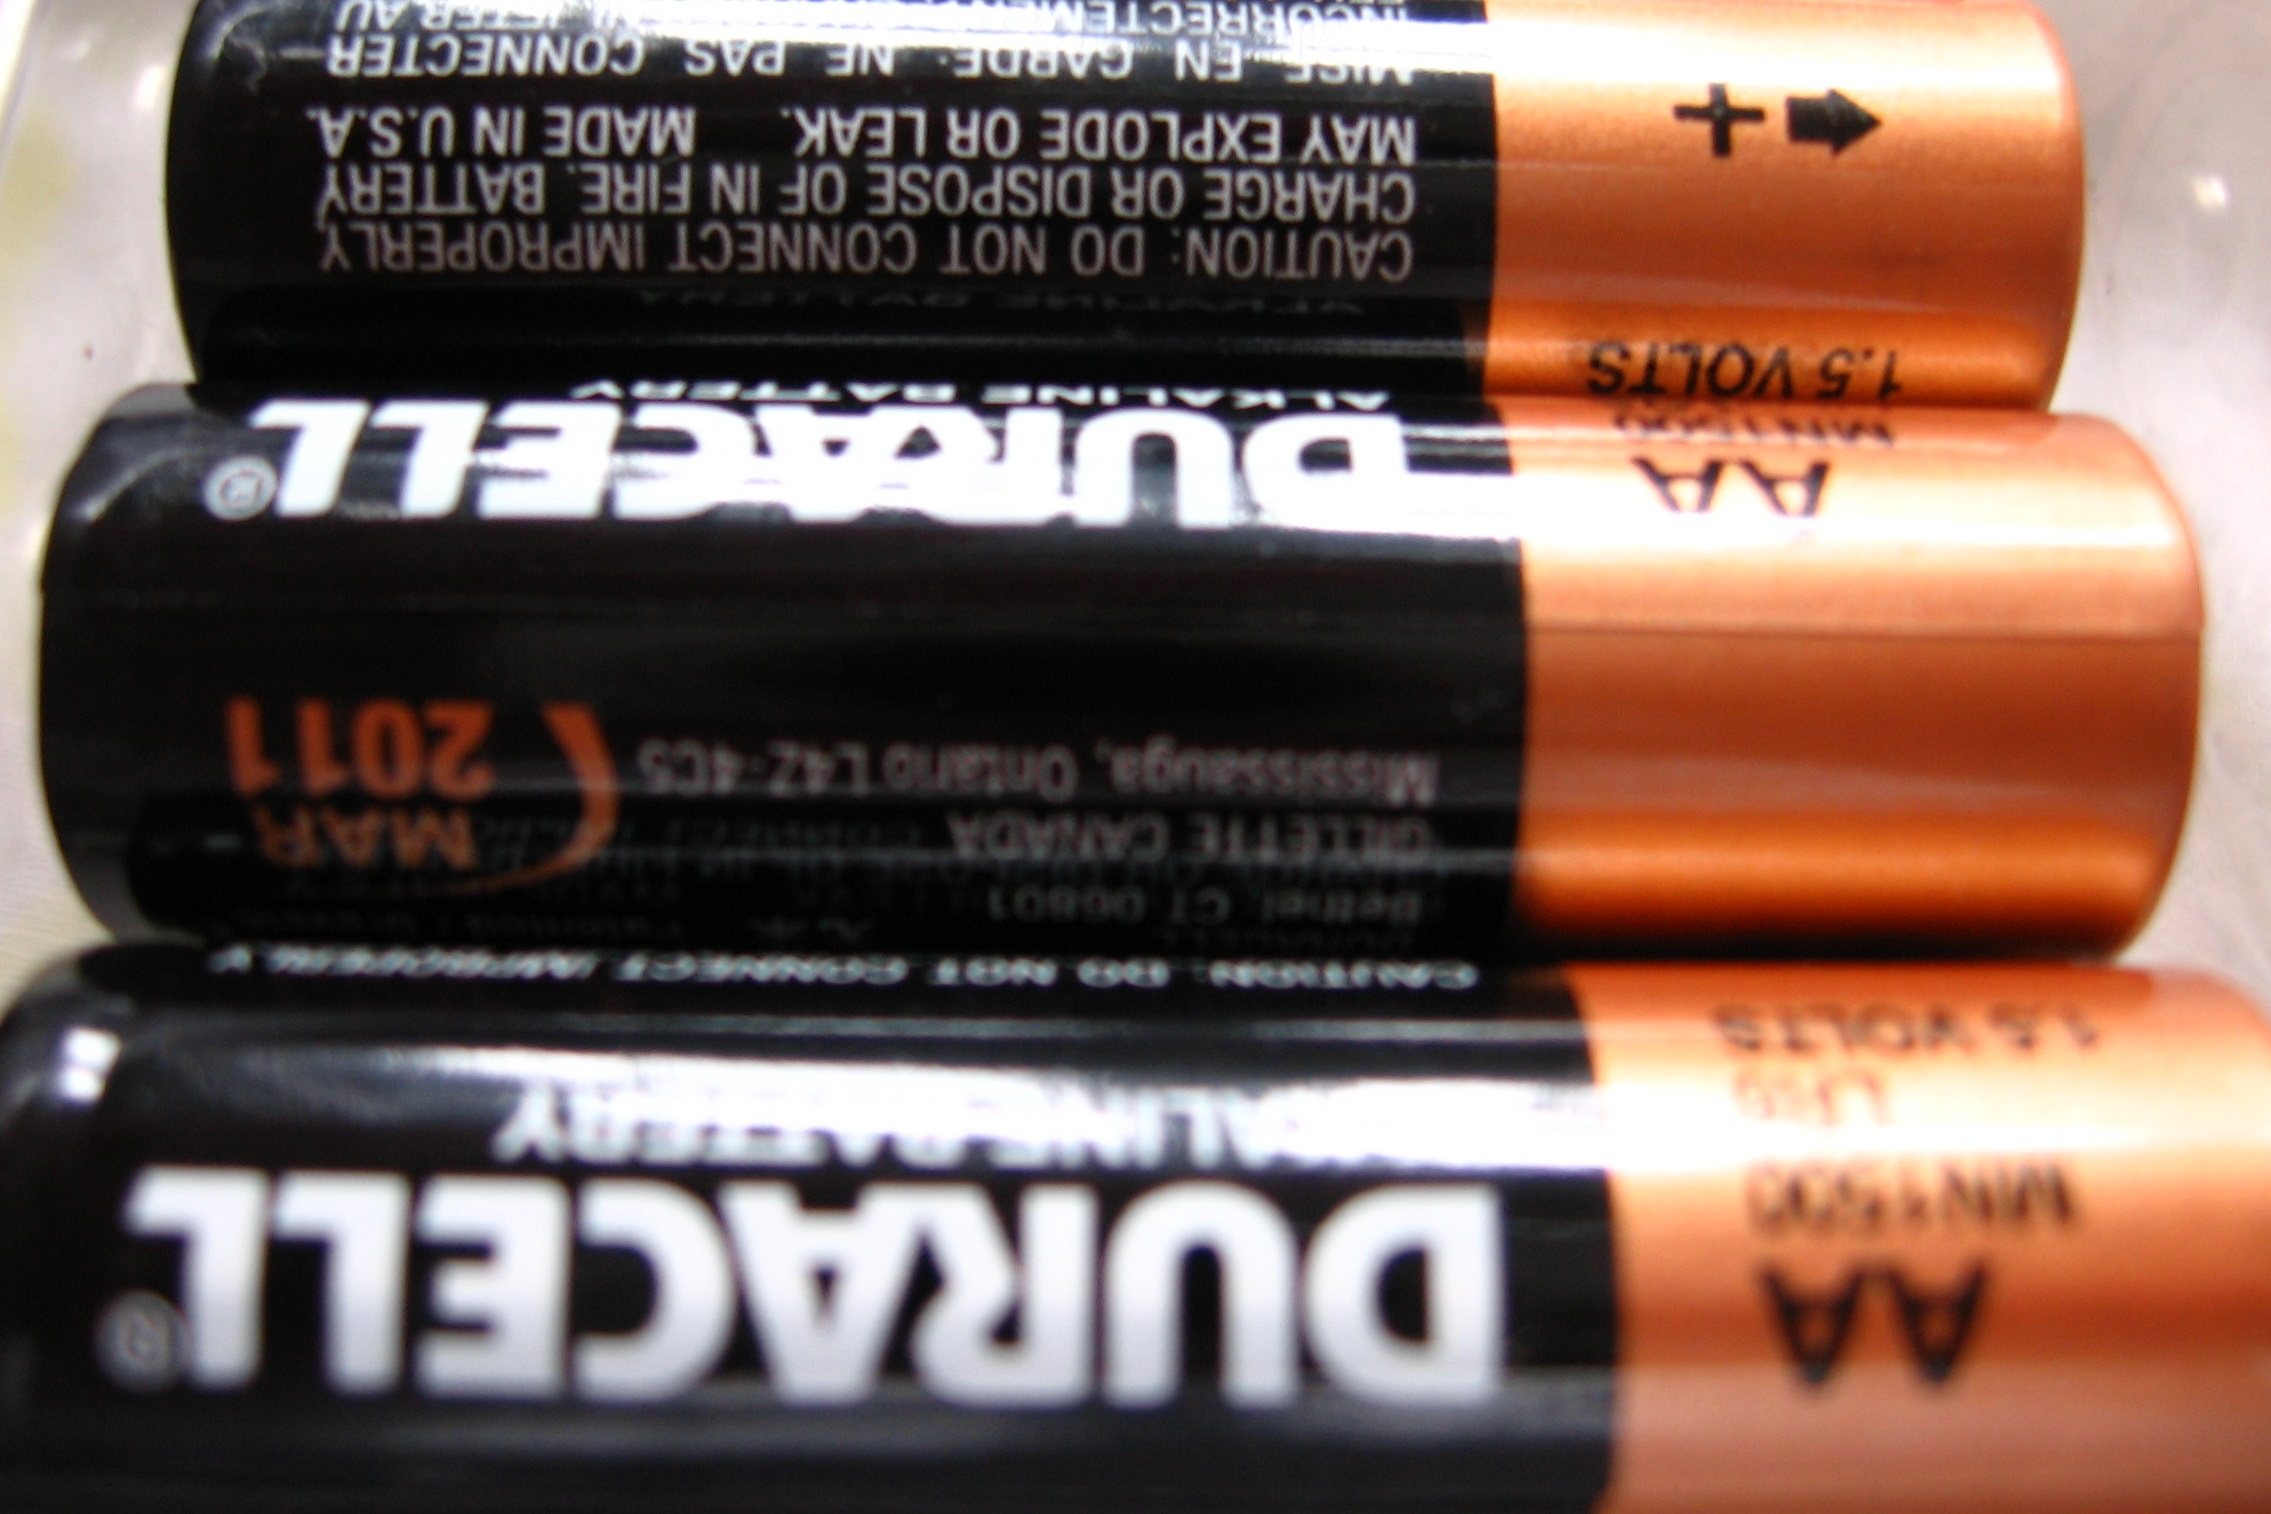
\includegraphics[width=2cm]{img/pile} & 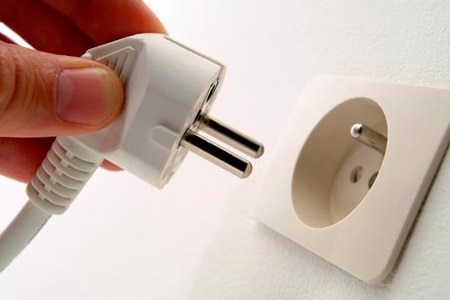
\includegraphics[width=2cm]{img/priseelectrique} & 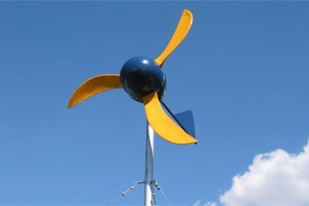
\includegraphics[width=2cm]{img/eolien} & 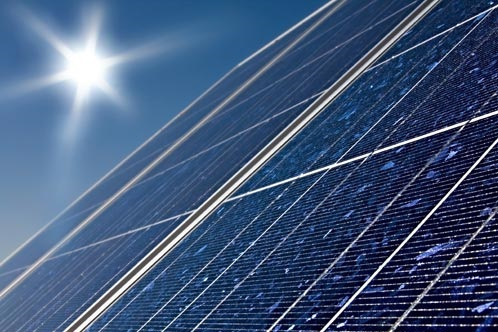
\includegraphics[width=2cm]{img/solaire} \\ \hline
Carburant & Pneumatique & Pile à hydrogène & Autres \\ 
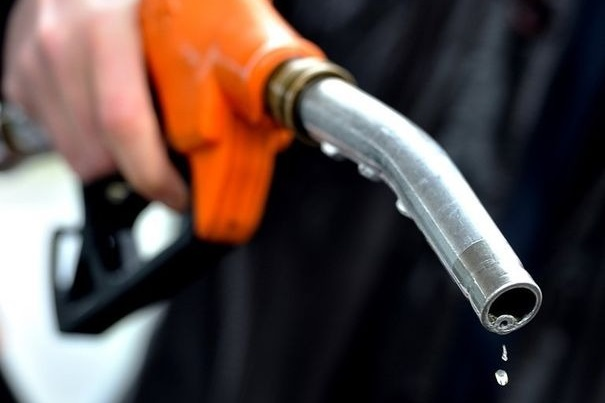
\includegraphics[width=2cm]{img/essence} & 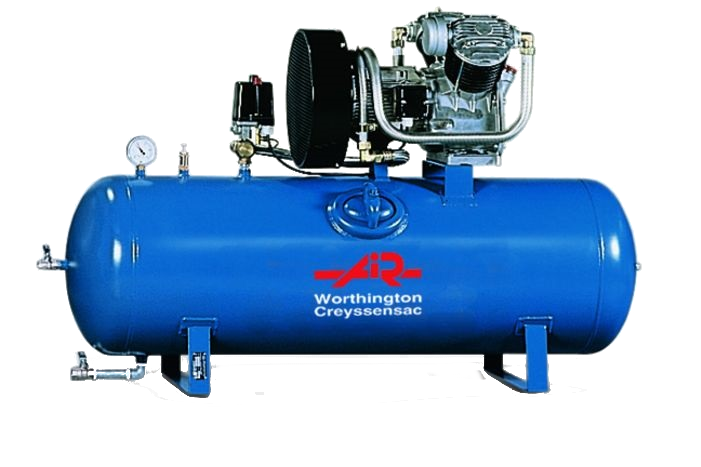
\includegraphics[width=2cm]{img/compresseur} & 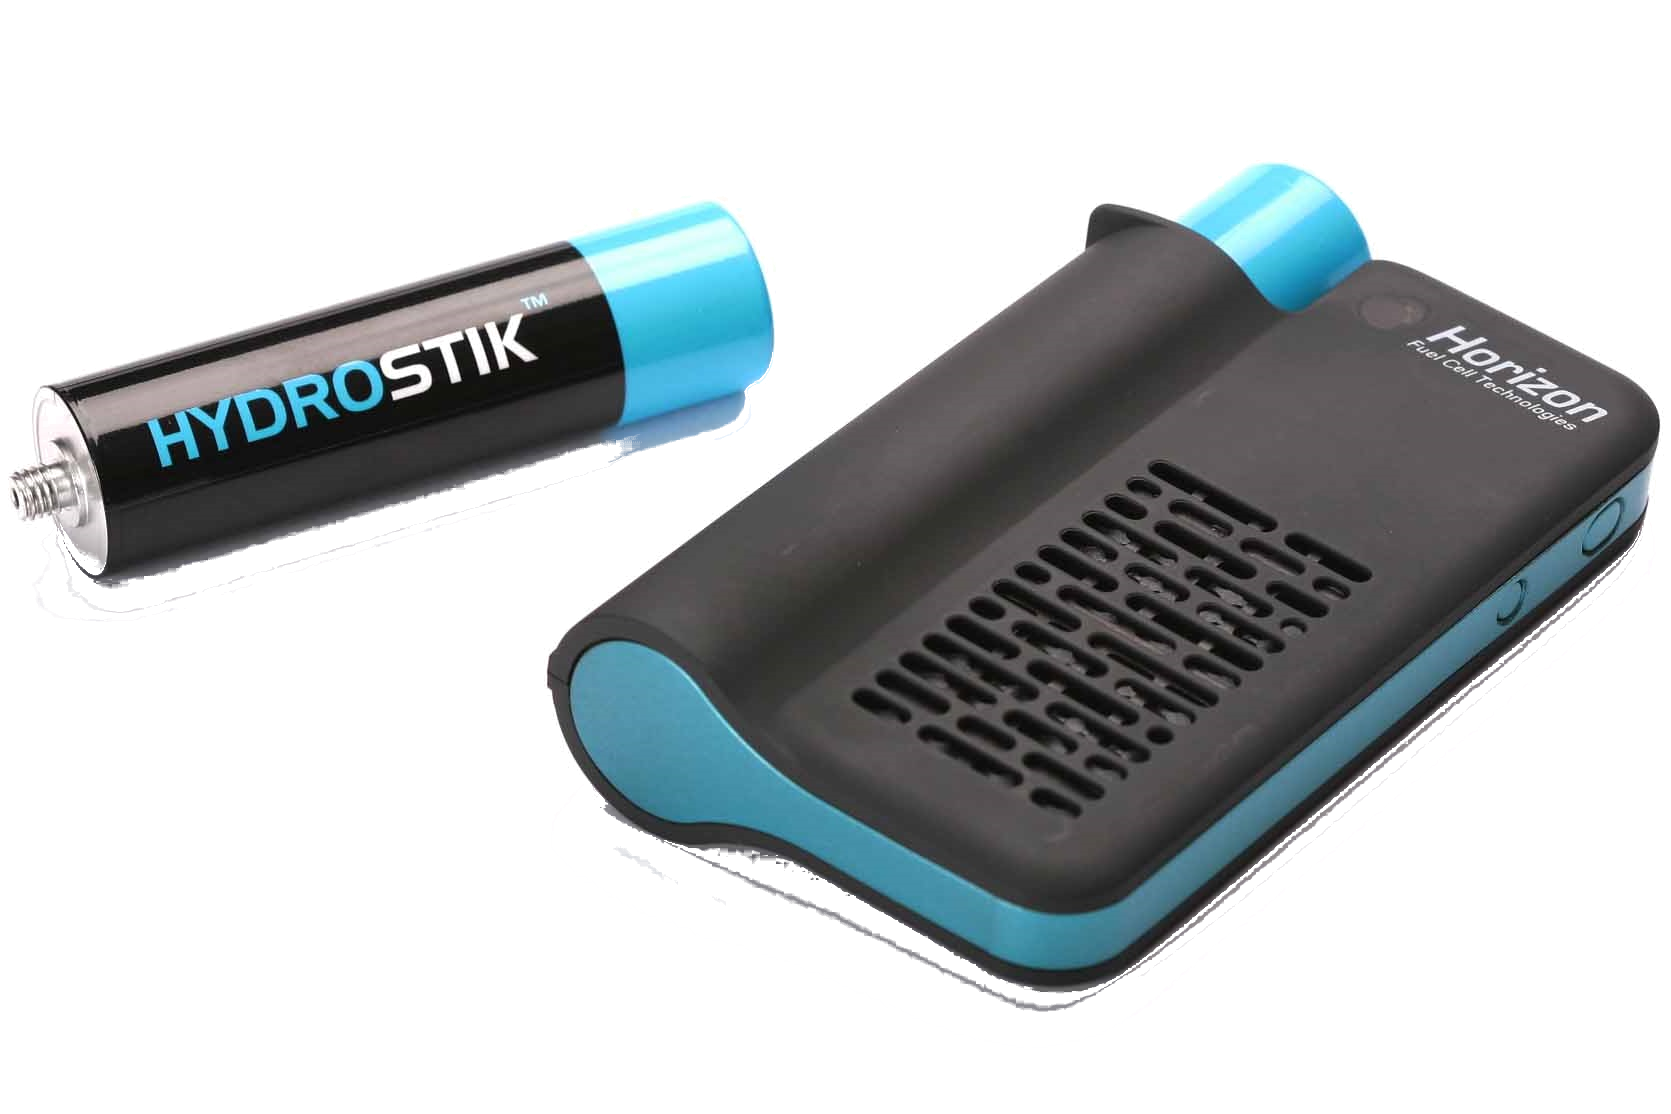
\includegraphics[width=2cm]{img/pile_combustible} & ... \\ \hline
\end{tabular}
\end{center}

\begin{rem}
\begin{minipage}{0.8\linewidth}
Cette énergie a parfois besoin d'être \textbf{adaptée} au système en utilisant un composant particulier (transformateur, redresseur, filtre,...) 
\end{minipage}
\hfill
\begin{minipage}{0.15\linewidth}
\centering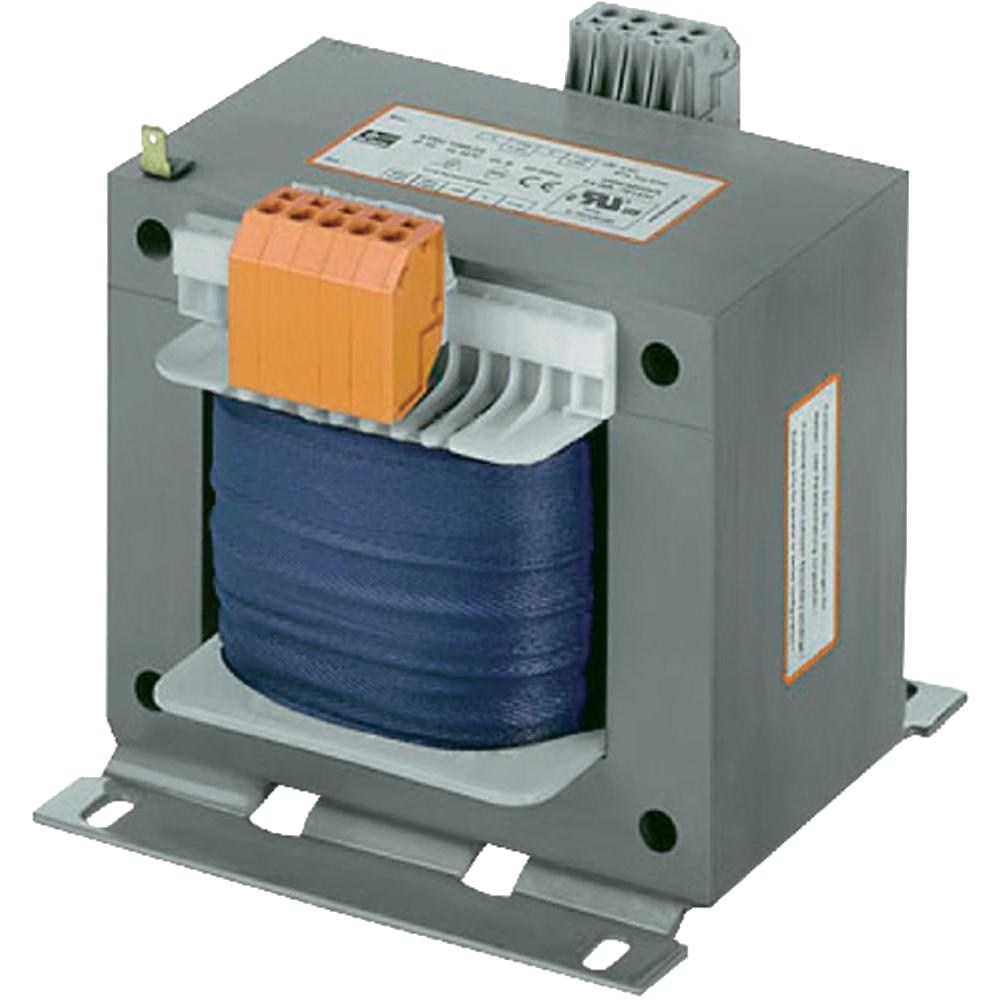
\includegraphics[width=0.7\linewidth]{img/transformateur}
\end{minipage}
\end{rem}
}}

{\frame{
\frametitle{Distribuer/moduler}

La \textbf{distribution} d'énergie à l'actionneur signifie que le \textbf{préactionneur} est une sorte d'\og interrupteur \fg sur le circuit reliant la source d'énergie de puissance à l'actionneur.

Le préactionneur est le constituant dont le rôle est de distribuer/moduler l'\textbf{énergie de puissance} utile aux actionneurs sur ordre de la \textbf{partie commande}.

~\

\begin{minipage}{0.48\linewidth}
Les distributeurs sont classés suivant :
\begin{itemize}
 \item Le type d'énergie distribuée,
 \item Le format de l'ordre de la commande.
\end{itemize}\end{minipage}
\hfill
\begin{minipage}{0.48\linewidth}
Distributeur tout ou rien (plus d'une position):
\begin{itemize}
 \item \textit{Monostable} : Une seule position stable. 
 \item \textit{Bistable} : Deux positions stables.
\end{itemize}
\end{minipage}

\begin{center}
\begin{tabular}{|c|c|c|}
\hline
\multicolumn{2}{|c|}{Énergie électrique} & Énergie pneumatique \\
\hline
Relais électrique & Variateur électrique & Distributeur pneumatique \\ 
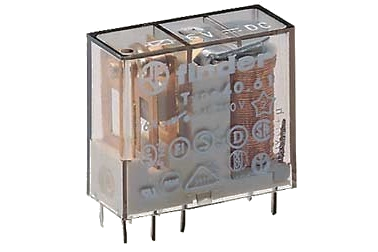
\includegraphics[width=2cm]{img/relais} & 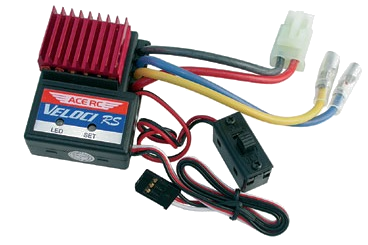
\includegraphics[width=2cm]{img/variateur} & 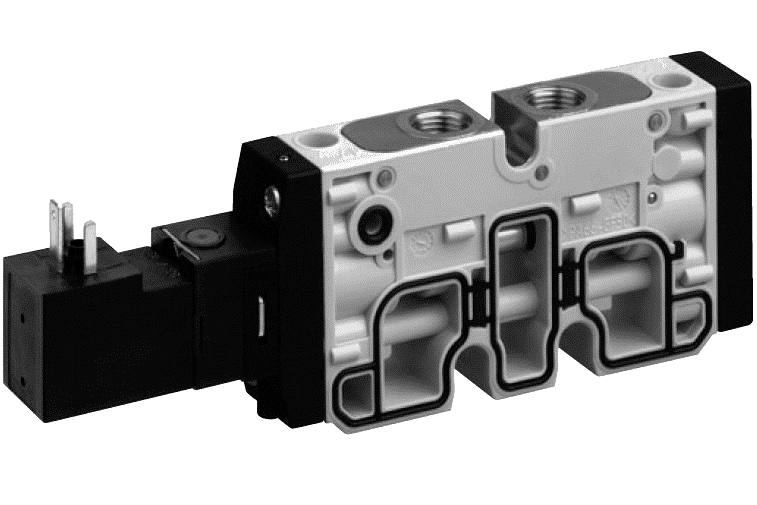
\includegraphics[width=2cm]{img/distributeur_pneumatique} \\ \hline
\end{tabular}
\end{center}
}}

{\frame{
\frametitle{Convertir}

La \textbf{conversion} de l'énergie est effectuée grâce à l'actionneur. Il convertit l'\textbf{énergie d'entrée} non directement utilisable par les effecteurs en une \textbf{énergie de sortie} utilisable par ces mécanismes pour obtenir une action définie.

\begin{itemize}
 \item L'énergie d'entrée non directement utilisable par les effecteurs peut être électrique, pneumatique ou hydraulique,
 \item L'énergie de sortie utilisable par ces mécanismes pour obtenir une action définie est généralement de l'énergie mécanique.
\end{itemize}

\begin{center}
\begin{tabular}{|c|c|c|c|}
\hline
\multicolumn{3}{|c|}{Énergie électrique} & Énergie pneumatique \\
\hline
Moteur rotatif & Moteur linéaire & Pompe & Vérin \\ 
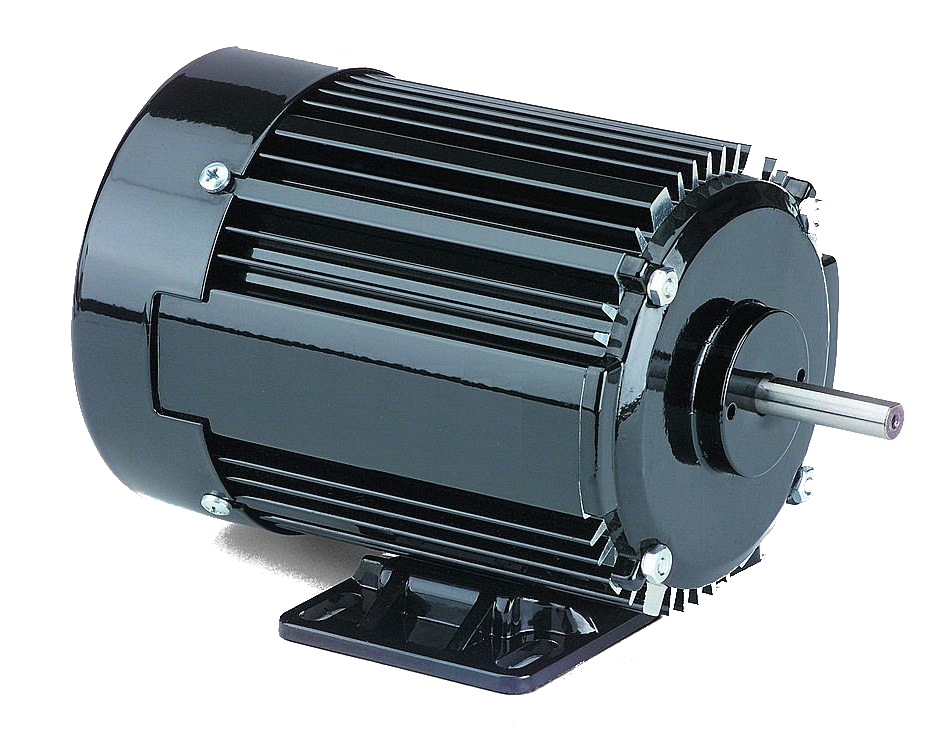
\includegraphics[width=2cm]{img/moteur_rotatif} & 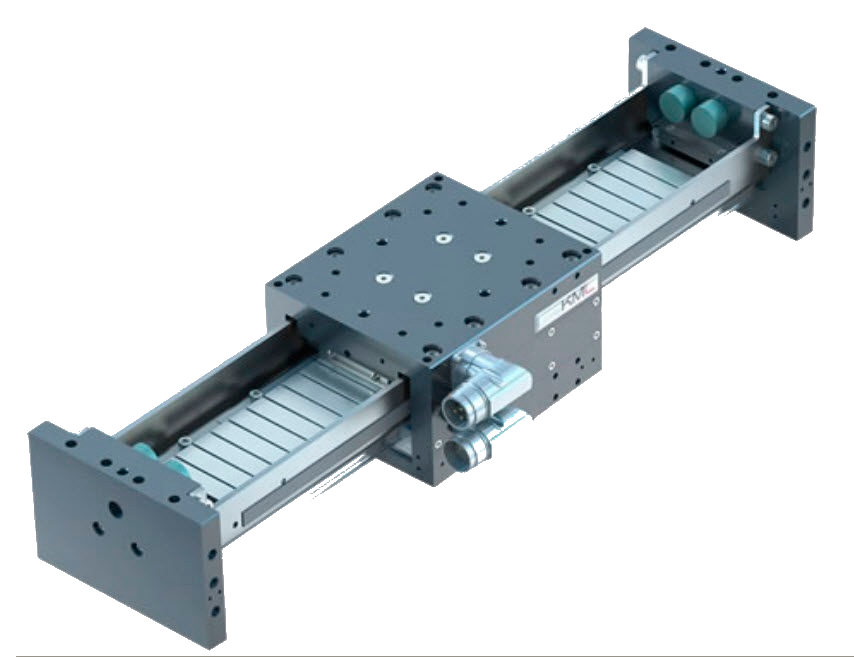
\includegraphics[width=2cm]{img/moteur_lineaire} & 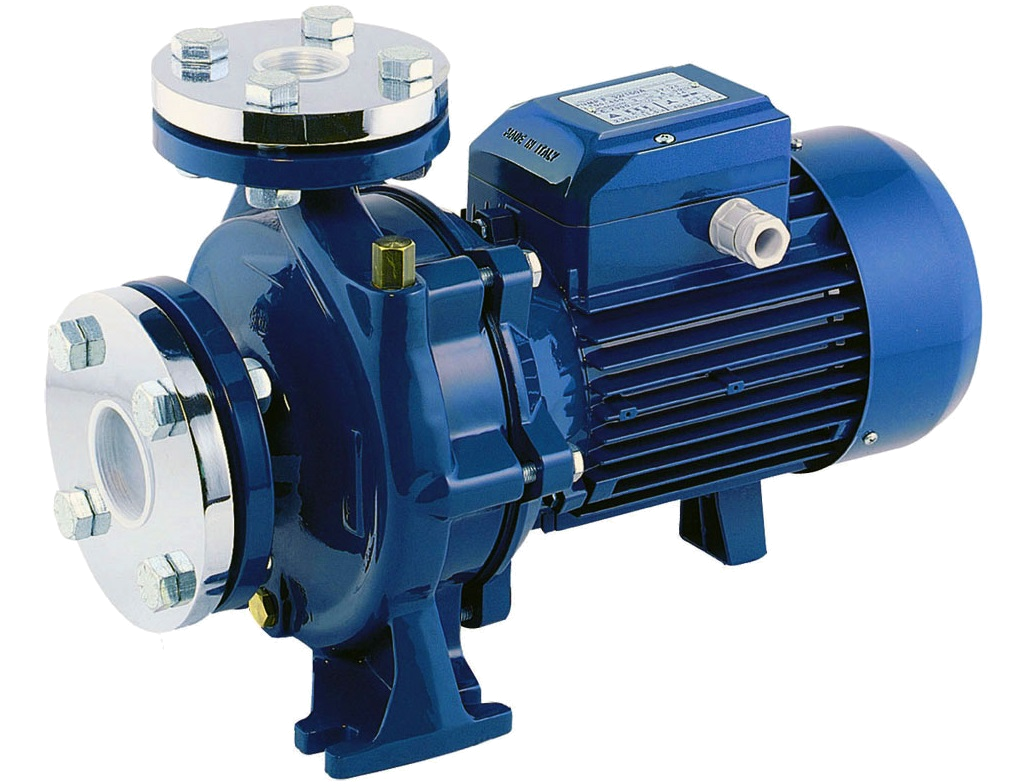
\includegraphics[width=2cm]{img/pompe}
& 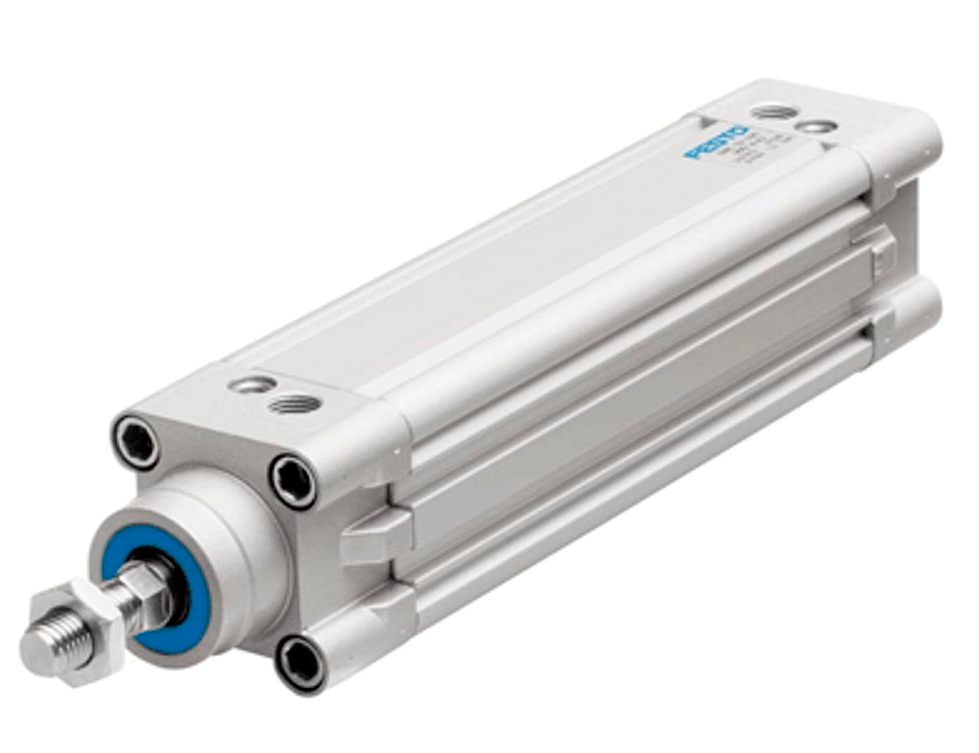
\includegraphics[width=2cm]{img/verin_pneumatique} \\ \hline
\end{tabular}
\end{center}
}}

{\frame{
\frametitle{Transmettre}

La \textbf{transmission} de l'énergie ne constitue qu'un \textbf{transport} de cette énergie, d'une \textbf{adaptation} mais il y a conservation du type d'énergie.

Dans la majorité des cas qui nous intéressent, l'énergie convertie par l'actionneur est de l'\textbf{énergie mécanique}. En conséquence, seuls les systèmes de transmission mécanique sont étudiés.

C'est la \textbf{cinématique} et les \textbf{degrés de liberté} du mécanisme qui vont permettre de transmettre le mouvement. Il faut tenir compte des mobilités utiles du mécanisme.

\begin{center}
\begin{tabular}{|c|c|c|}
\hline
\multicolumn{3}{|c|}{Énergie mécanique} \\
\hline
Poulie-courroie & Pignon-crémaillère & Engrenages \\ 
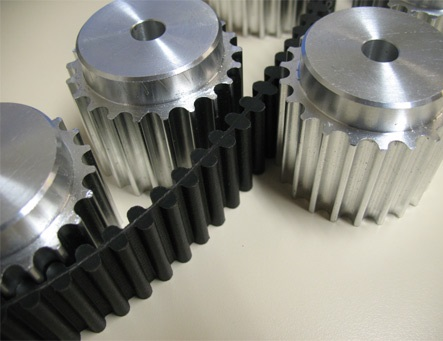
\includegraphics[width=2cm]{img/poulies} & 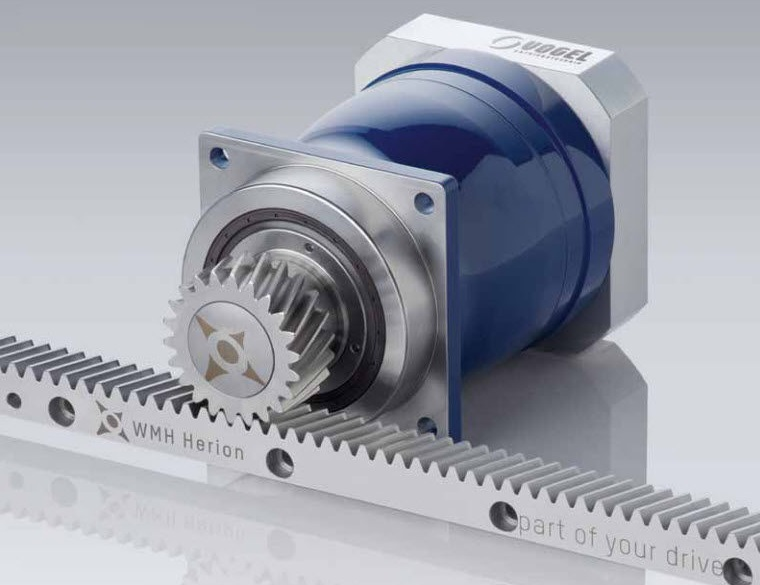
\includegraphics[width=2cm]{img/pignon} & 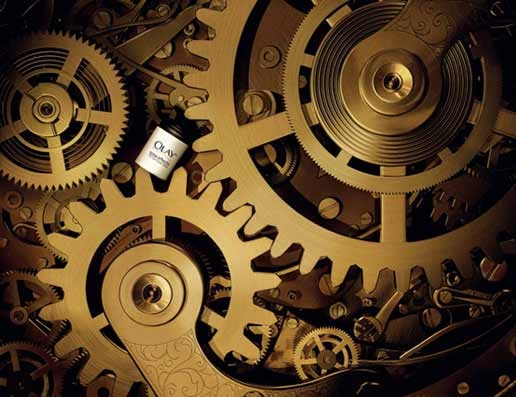
\includegraphics[width=2cm]{img/engrenages} \\ \hline
\end{tabular}
\end{center}
}}

{\frame{
\frametitle{Le schéma électrique}

Un \textbf{schéma de puissance} électrique représente, à l'aide de symboles graphiques, les fonctionnalités du circuit électrique réel.

\begin{minipage}{0.48\linewidth}
Commentaires :
\begin{itemize}
 \item Réseau de distribution électrique: \textbf{alimente} le circuit électrique du produit
 \item Sectionneur porte-fusibles: \textbf{isole} le circuit amont du circuit aval
 \item Fusibles: \textbf{protègent} contre les courts-circuits
 \item Contacteur : \textbf{distribue} l'énergie sur ordre de la chaîne d'information
 \item Relais thermique : \textbf{protège} contre les surcharges du moteur (réglage de sensibilité possible
\end{itemize}\end{minipage}
\hfill
\begin{minipage}{0.48\linewidth}
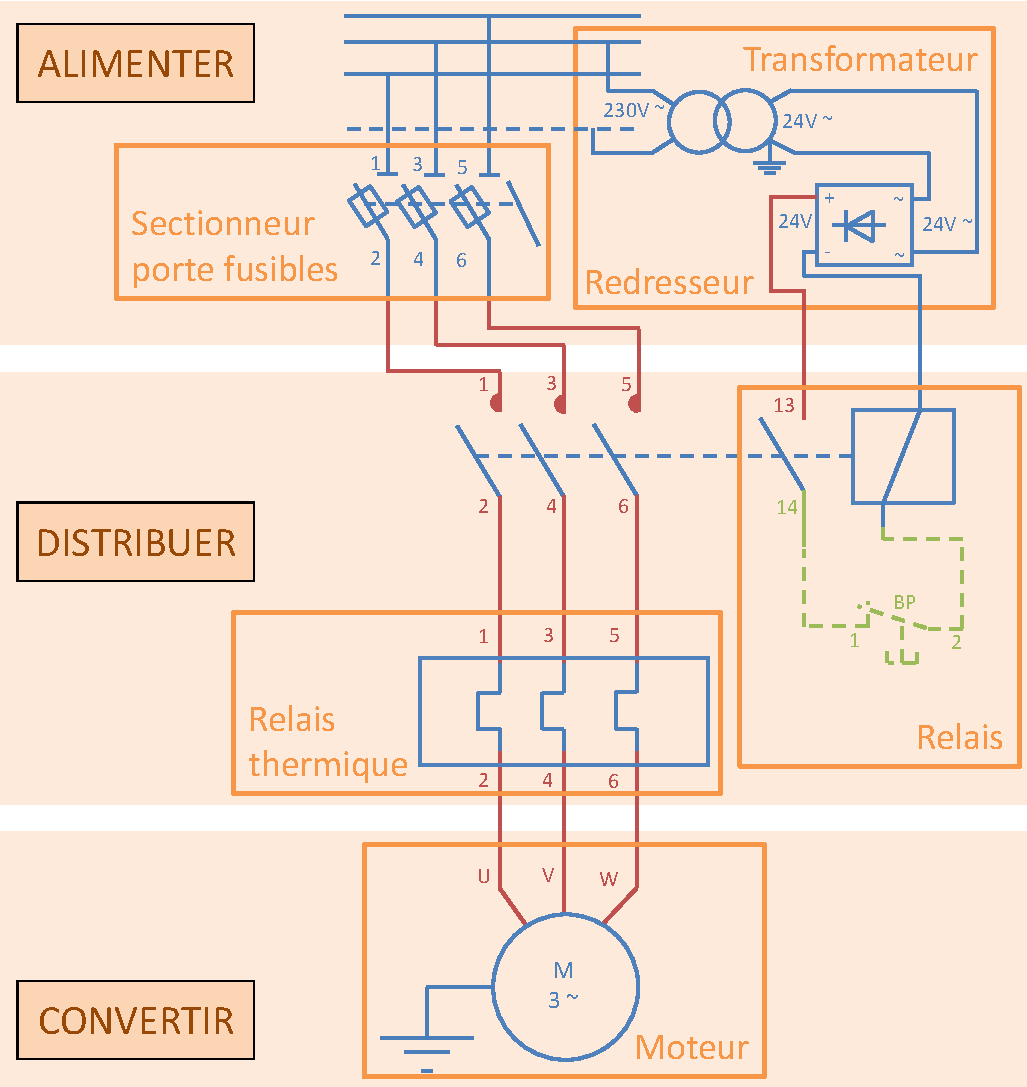
\includegraphics[width=\linewidth]{img/schema_elec}
\end{minipage}
}}


{\frame{
\frametitle{Le schéma pneumatique}

Un \textbf{schéma de puissance} pneumatique représente, à l'aide de symboles graphiques, les fonctionnalités du circuit pneumatique réel.

\begin{minipage}{0.48\linewidth}

Commentaires :
\begin{itemize}
 \item Réseau de distribution: \textbf{alimente} le circuit pneumatique en énergie
 \item Régleur de débit unidirectionnel (clapet de non retour avec étranglement réglable): \textbf{règle} la vitesse du vérin
 \item Distributeur : \textbf{distribue} l'air comprimé sur ordre de la chaîne d'information
 \item Le vérin: \textbf{convertit} l'énergie pneumatique en énergie mécanique
\end{itemize}\end{minipage}
\hfill
\begin{minipage}{0.48\linewidth}
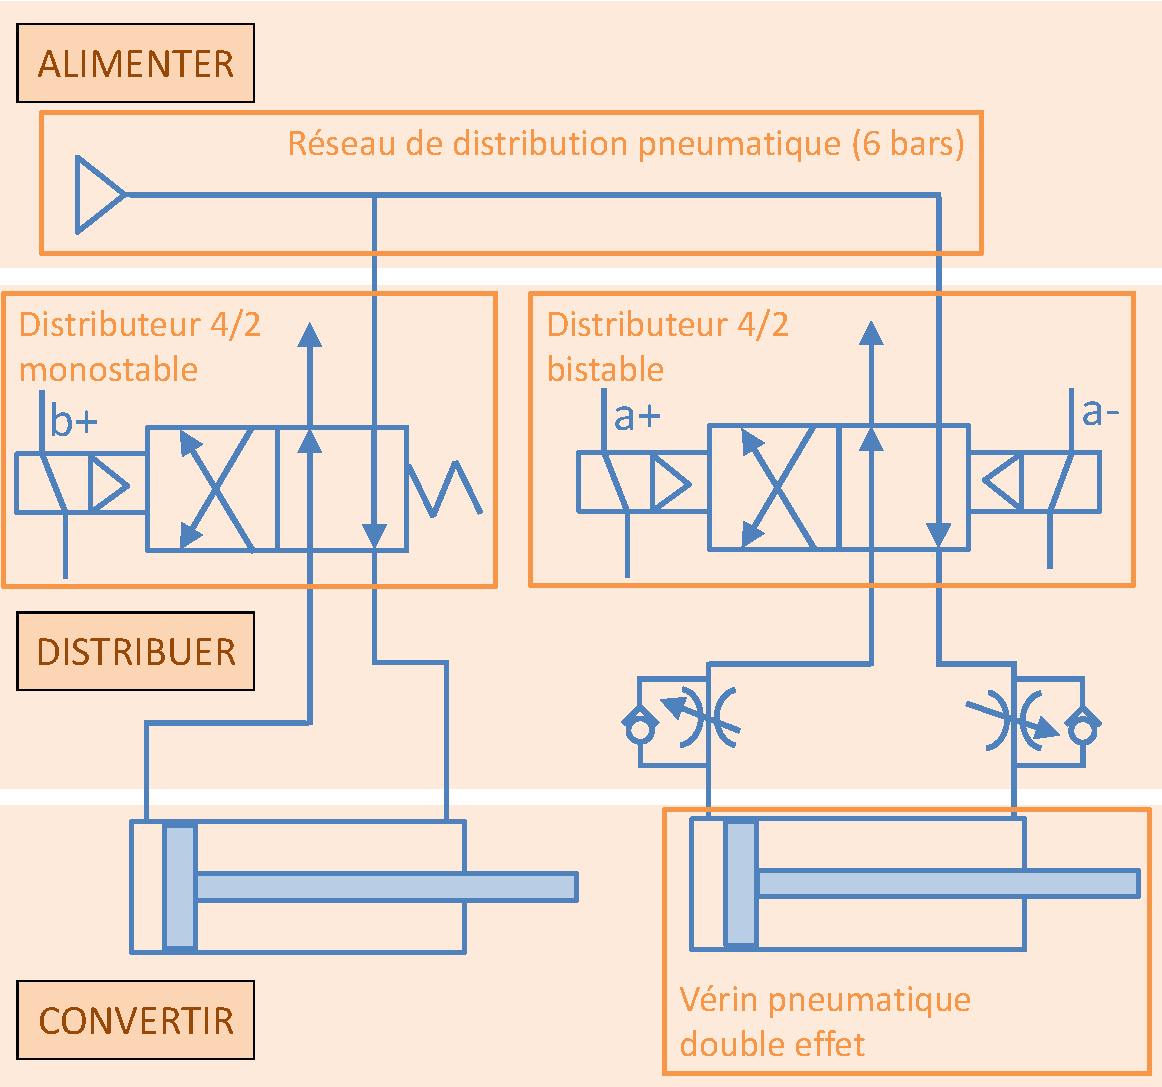
\includegraphics[width=\linewidth]{img/schema_pneu}
\end{minipage}
}}

\section{Les unités}

\ifdef{\public}{
\begin{frame}
\frametitle{Table des matières}
\tableofcontents[currentsection]
\end{frame}}

{\frame{
\frametitle{Le Système International d'unités}

Le nom \textbf{Système international d'unités}, et l'abréviation \textbf{SI}, ont été établis par la 11e Conférence générale des poids et mesures (CGPM) en 1960.

Les \textbf{grandeurs} de base sont, par convention, considérées comme \textbf{indépendantes}.

\vfill

\begin{center}
\begin{tabular}{|c|c|c|}
\hline
Nom de la grandeur de base & Nom l'unité SI de base & Symbole \\
\hline
Longueur & \ifdef{\public}{Mètre}{..........} & \ifdef{\public}{$m$}{..........} \\
\hline
Masse & \ifdef{\public}{Kilogramme}{..........} & \ifdef{\public}{$kg$}{..........} \\
\hline
Durée & \ifdef{\public}{Seconde}{..........} & \ifdef{\public}{$s$}{..........} \\
\hline
Courant électrique & \ifdef{\public}{Ampère}{..........} & \ifdef{\public}{$A$}{..........} \\
\hline
Température & \ifdef{\public}{Kelvin}{..........} & \ifdef{\public}{$K$}{..........} \\
\hline
Quantité de matière & \ifdef{\public}{Mole}{..........} & \ifdef{\public}{$mol$}{..........} \\
\hline
Intensité lumineuse & \ifdef{\public}{Candela}{..........} & \ifdef{\public}{$cd$}{..........} \\
\hline
\end{tabular}
\end{center}
}}


{\frame{
\frametitle{Exemples d'unités SI dérivées cohérentes}

Des unités sont \textbf{dérivées} des unités SI. 

\vfill

\begin{center}
\begin{tabular}{|c|c|c|}
\hline
Nom de la grandeur de base & Nom l'unité SI de base & Symbole \\
\hline
Superficie & \ifdef{\public}{Mètre carré}{..........} & \ifdef{\public}{$m^2$}{..........} \\
\hline
Volume & \ifdef{\public}{Mètre cube}{..........} & \ifdef{\public}{$m^3$}{..........} \\
\hline
Vitesse & \ifdef{\public}{Mètre par seconde}{..........} & \ifdef{\public}{$m.s^{-1}$}{..........} \\
\hline
Accélération & \ifdef{\public}{Mètre par seconde carré}{..........} & \ifdef{\public}{$m.s^{-2}$}{..........} \\
\hline
Masse linéique & \ifdef{\public}{Kilogramme par mètre}{..........} & \ifdef{\public}{$kg.m^{-1}$}{..........} \\
\hline
Masse surfacique & \ifdef{\public}{Kilogramme par mètre carré}{..........} & \ifdef{\public}{$kg.m^{-2}$}{..........} \\
\hline
Masse volumique & \ifdef{\public}{Kilogramme par mètre cube}{..........} & \ifdef{\public}{$kg.m^{-3}$}{..........} \\
\hline
\end{tabular}
\end{center}
}}

{\frame{
\frametitle{Vérification de l'homogénéité}

En physique et Sciences Industrielles, les résultats de calculs doivent \textbf{toujours être vérifiés} à l'aide de la vérification de l'\textbf{homogénéité}.

Le principe de cette vérification et de \textbf{comparer} les unités des grandeurs présentes dans une équation.

La \textbf{dimension} d'une \textbf{grandeur} X s'écrit comme suit: [X].

Exemples:
\begin{itemize}
 \item Vitesse: $[v]=L/T$ (exemple: $m.s^{-1}$),
 \item Masse volumique: $[\rho]=M/L^3$ (exemple=$kg.m^{-3}$).
\end{itemize}

Ainsi, il \textbf{suffit} de connaître quelques formules pour retrouver les unités SI des grandeurs les plus utilisées.

}}

{\frame{
\frametitle{Exemples d'unités SI dérivées cohérentes}

Des unités sont dérivées des unités SI, elles peuvent avoir des \textbf{noms spéciaux}. 

\vfill

\begin{center}
\begin{tabular}{|c|c|c|c|c|}
\hline
Nom de la & Nom de & Symbole & Formule & Unité SI \\
grandeur dérivée & l'unité dérivée &   & mnémonique &  \\
\hline
Angle plan & Radian & rad & $\theta=\frac{\pi.\Theta}{180}$ & .......... \\
\hline
Fréquence & Hertz & Hz & .......... & .......... \\
\hline
Force & Newton & N & .......... & .......... \\
\hline
Pression & Pascal & Pa & .......... & .......... \\
\hline
Énergie & Joule & J & .......... & .......... \\
\hline
Puissance & Watt & W & .......... & .......... \\
\hline
\end{tabular}
\end{center}
}}

\ifdef{\public}{{\frame{
\frametitle{Exemples d'unités SI dérivées cohérentes}

Des unités sont dérivées des unités SI, elles peuvent avoir des \textbf{noms spéciaux}. 

\vfill

\begin{center}
\begin{tabular}{|c|c|c|c|c|}
\hline
Nom de la & Nom de & Symbole & Formule & Unité SI \\
grandeur dérivée & l'unité dérivée &   & mnémonique &  \\
\hline
Angle plan & Radian & rad & $\theta=\frac{\pi.\Theta}{180}$ & $1$\\
\hline
Fréquence & Hertz & Hz & $f=\frac{1}{T}$& $s^{-1}$\\
\hline
Force & Newton & N & $P=m.g$& $m.kg.s^{-2}$\\
\hline
Pression & Pascal & Pa & $F=P.S$& $m^{-1}.kg.s^{-2}$\\
\hline
Énergie & Joule & J & $E=\frac{1}{2}m.v^2$& $m^2.kg.s^{-2}$\\
\hline
Puissance & Watt & W & $P=F.V=C.\Omega$& $m^2.kg.s^{-3}$\\
\hline
\end{tabular}
\end{center}
}}}

{\frame{
\frametitle{La décomposition d'un système}

\begin{savoir}

Vous devez être capables de retrouver les composants de la chaîne d'énergie dans un système.

\begin{itemize}
 \item Quelle énergie est utilisée par le système ?
 \item Quels sont les états possibles des actionneurs ?
 \item A quelle unité est associée une grandeur ?
\end{itemize}
\end{savoir}

\begin{prob}

La chaîne d'énergie ne permet de fournir au système que sa puissance.
\begin{itemize}
 \item \textit{Problème: Comment gérer le comportement du système}
 \item \textbf{Perspectives}: Reconnaître les éléments important d'une chaîne d'information.
\end{itemize}
\end{prob}
}}

\section{La chaîne d'information}

\ifdef{\public}{
\begin{frame}
\frametitle{Table des matières}
\tableofcontents[currentsection]
\end{frame}}

{\frame{
\frametitle{Les chaînes d'énergie et d'information}

Sur un \textbf{système complexe}, il est souvent nécessaire de \textbf{décomposer} son étude en plusieurs parties. Il existe plusieurs possibilité pour effectuer cette décomposition, celle qui va être vue maintenant revient à effectuer une isolation des \textbf{chaînes fonctionnelles}.

\ifdef{\public}{\begin{center}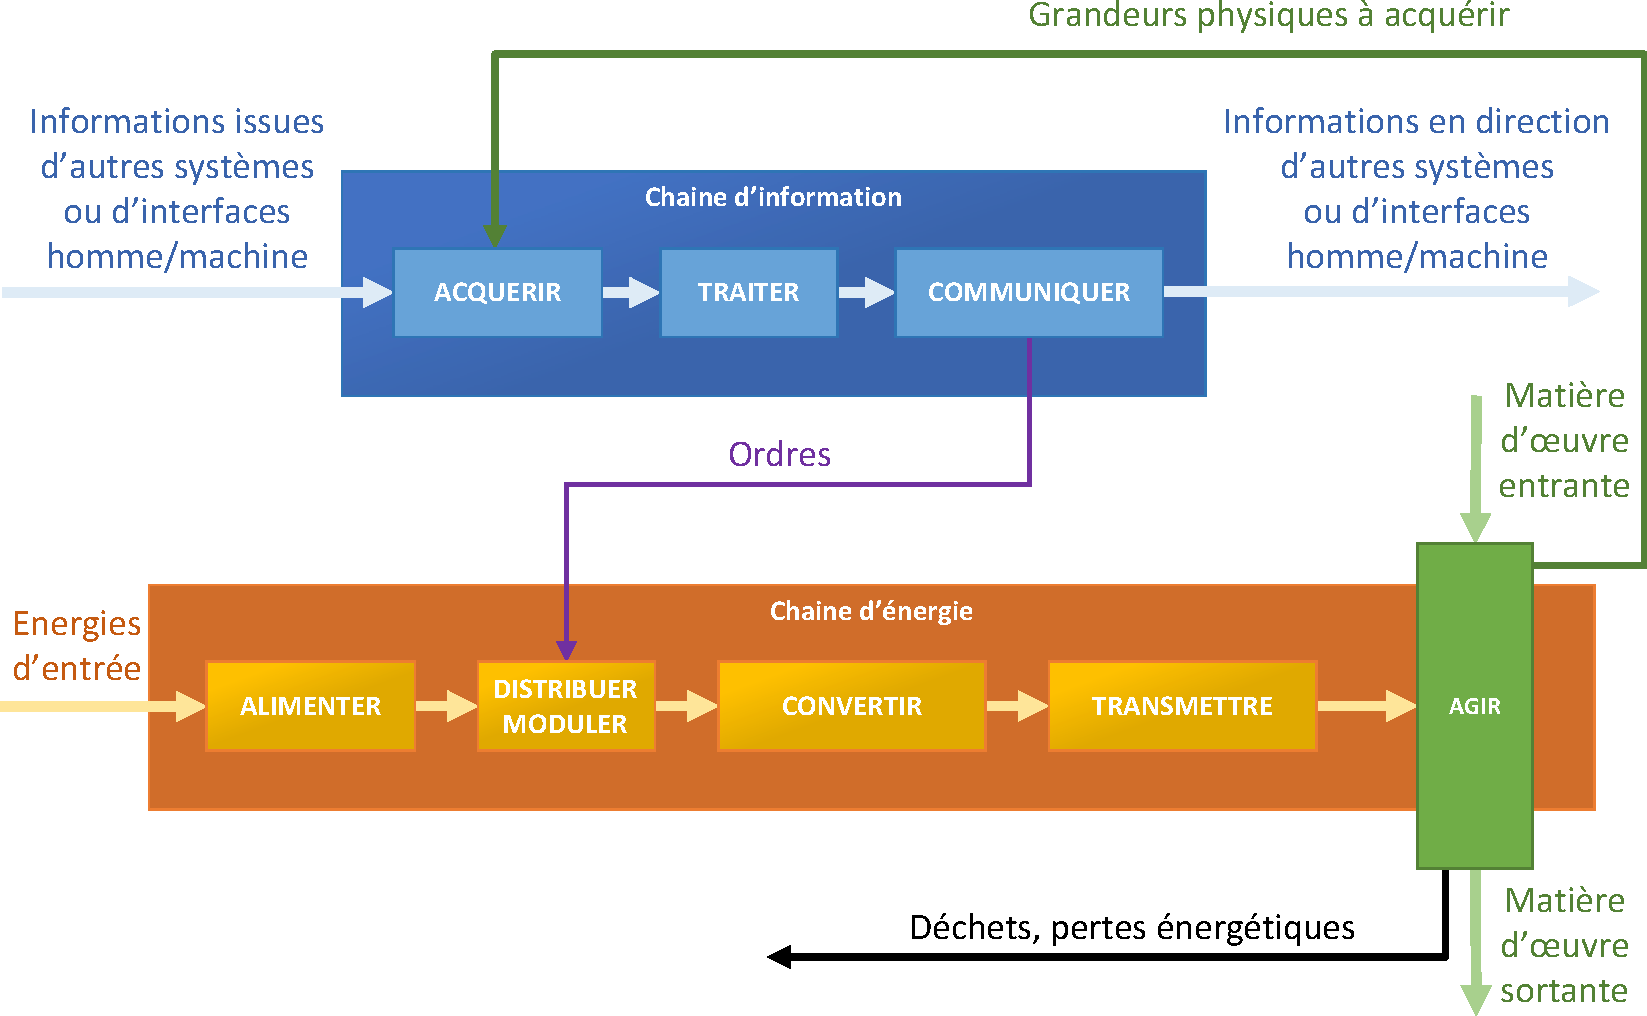
\includegraphics[width=0.8\linewidth]{img/Chaines}\end{center}}
{\begin{center}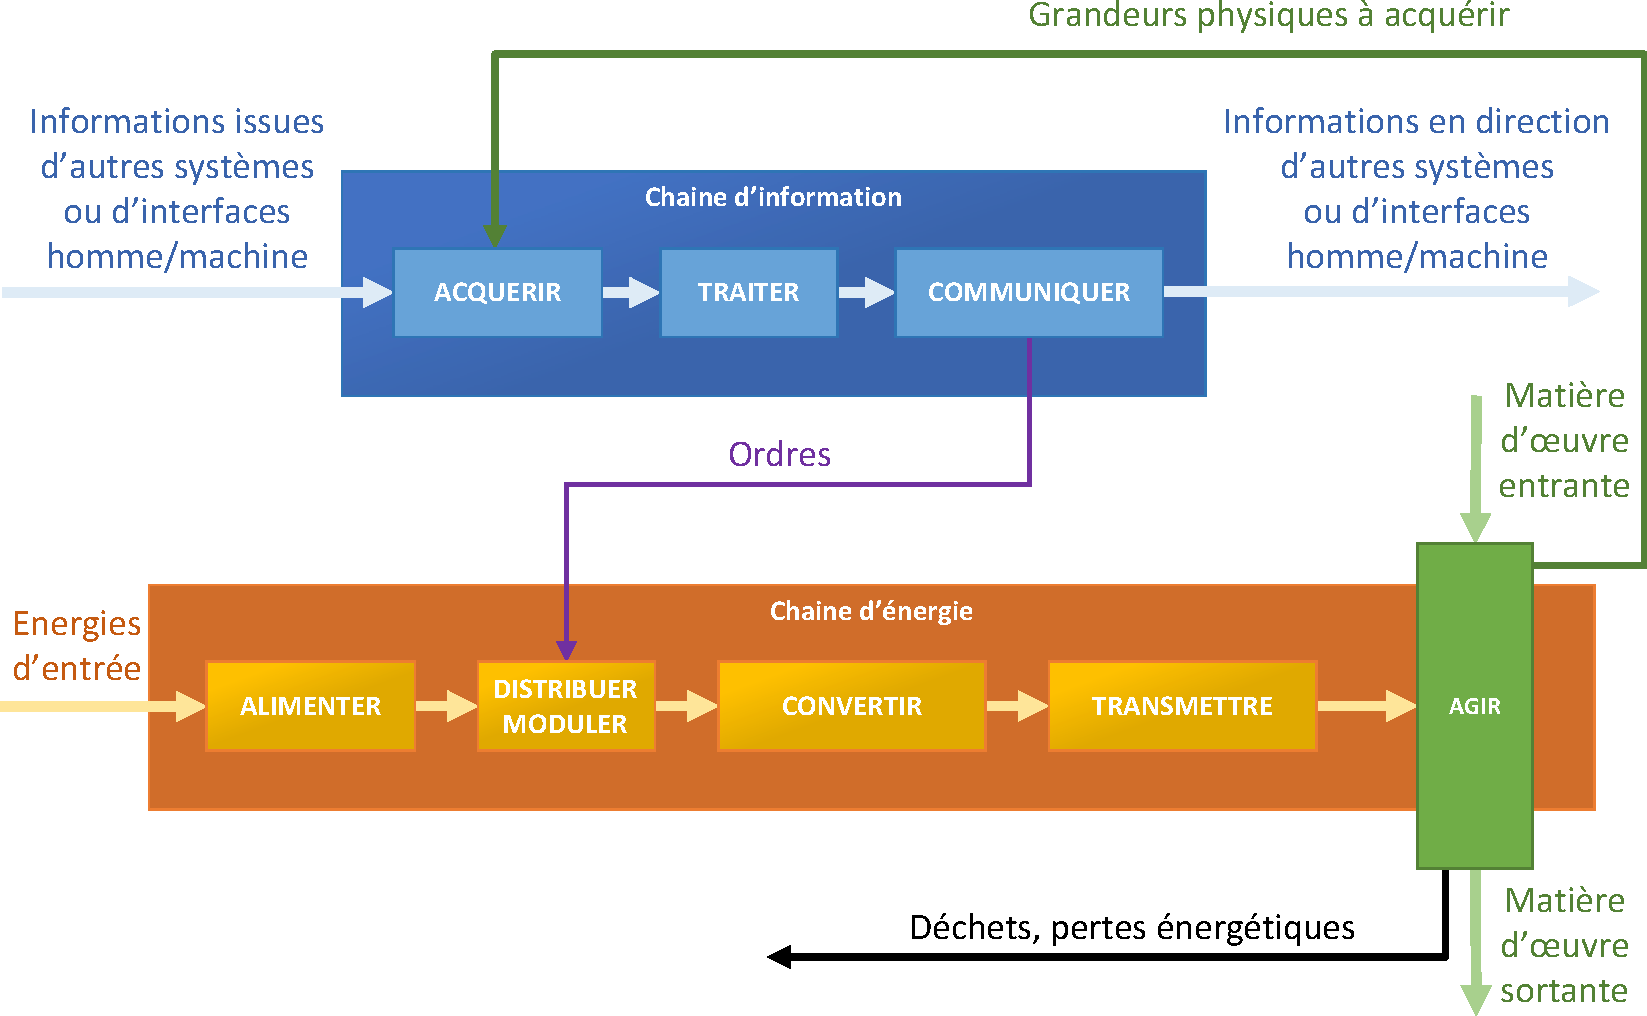
\includegraphics[width=0.8\linewidth]{img/Chaines}\end{center}}

}}


{\frame{
\frametitle{La chaîne d'information}

C'est par la \textbf{chaîne d'information} que transite les \textbf{messages} nécessaires au système pour fonctionner.

\ifdef{\public}{\begin{center}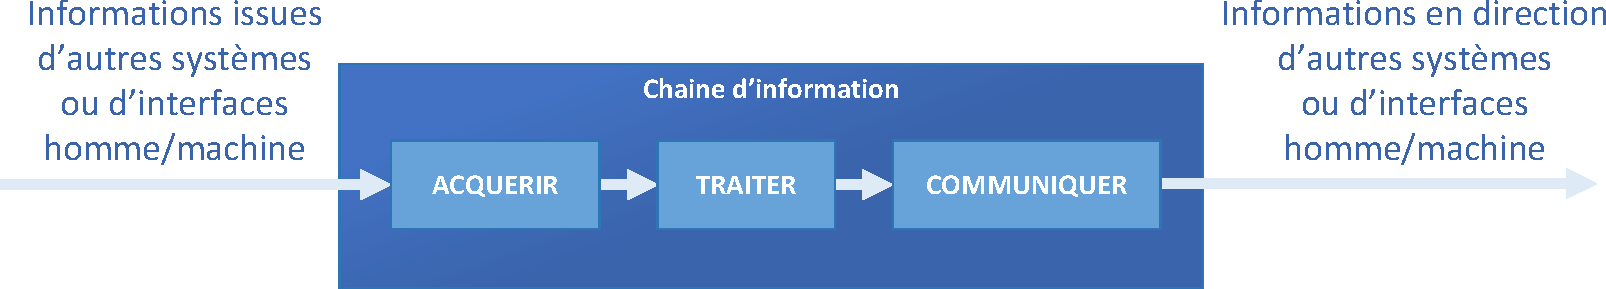
\includegraphics[width=0.8\linewidth]{img/Chaine_info}\end{center}}
{\begin{center}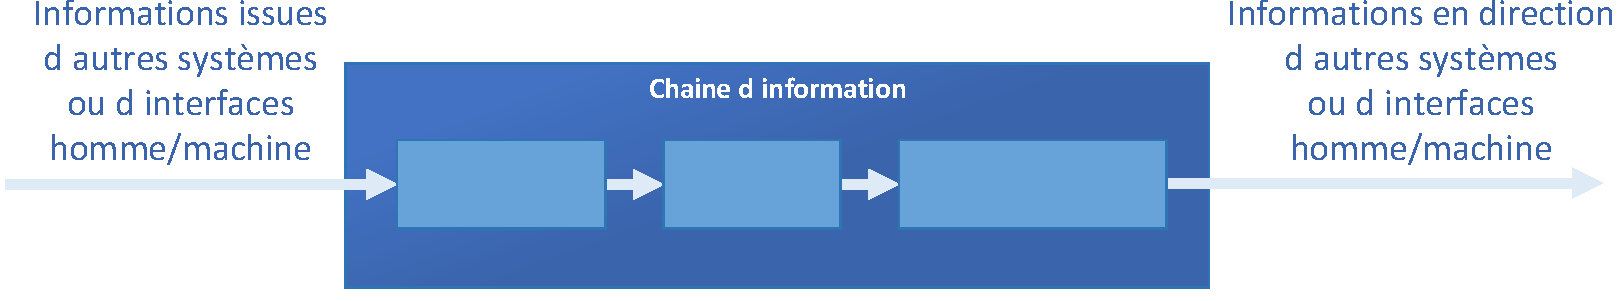
\includegraphics[width=0.8\linewidth]{img/Chaine_info_vide}\end{center}}

Nous allons détailler les fonctions de cette chaîne:
\begin{itemize}
 \item Acquérir,
 \item Traiter,
 \item Communiquer. 
\end{itemize}

}}

{\frame{
\frametitle{Nature de l'information}

\begin{itemize}
 \item \textbf{Logique}: Une information de nature \textbf{logique} est une information qui ne peut prendre que \textbf{2 états} (vrai ou faux, 0 ou 1, état haut ou état bas), on parle également d'information \textit{Tout Ou Rien}. Cette information sera transmise par un \textbf{signal logique}.
 \item \textbf{Analogique}: Une information de nature \textbf{analogique} est une information dont l'état peut varier de manière \textbf{continue} entre une valeur maximale et une valeur minimale. Cette information sera transmise par un \textbf{signal analogique}.
 \item \textbf{Numérique}: Une information de nature \textbf{numérique} est une information qui peut prendre un nombre \textbf{défini} (discret) de valeurs entre une valeur maximale et une valeur minimale. Cette information sera transmise par plusieurs \textbf{signaux logiques}.
\end{itemize}

\begin{center}
	\begin{tabular}{c c c}
	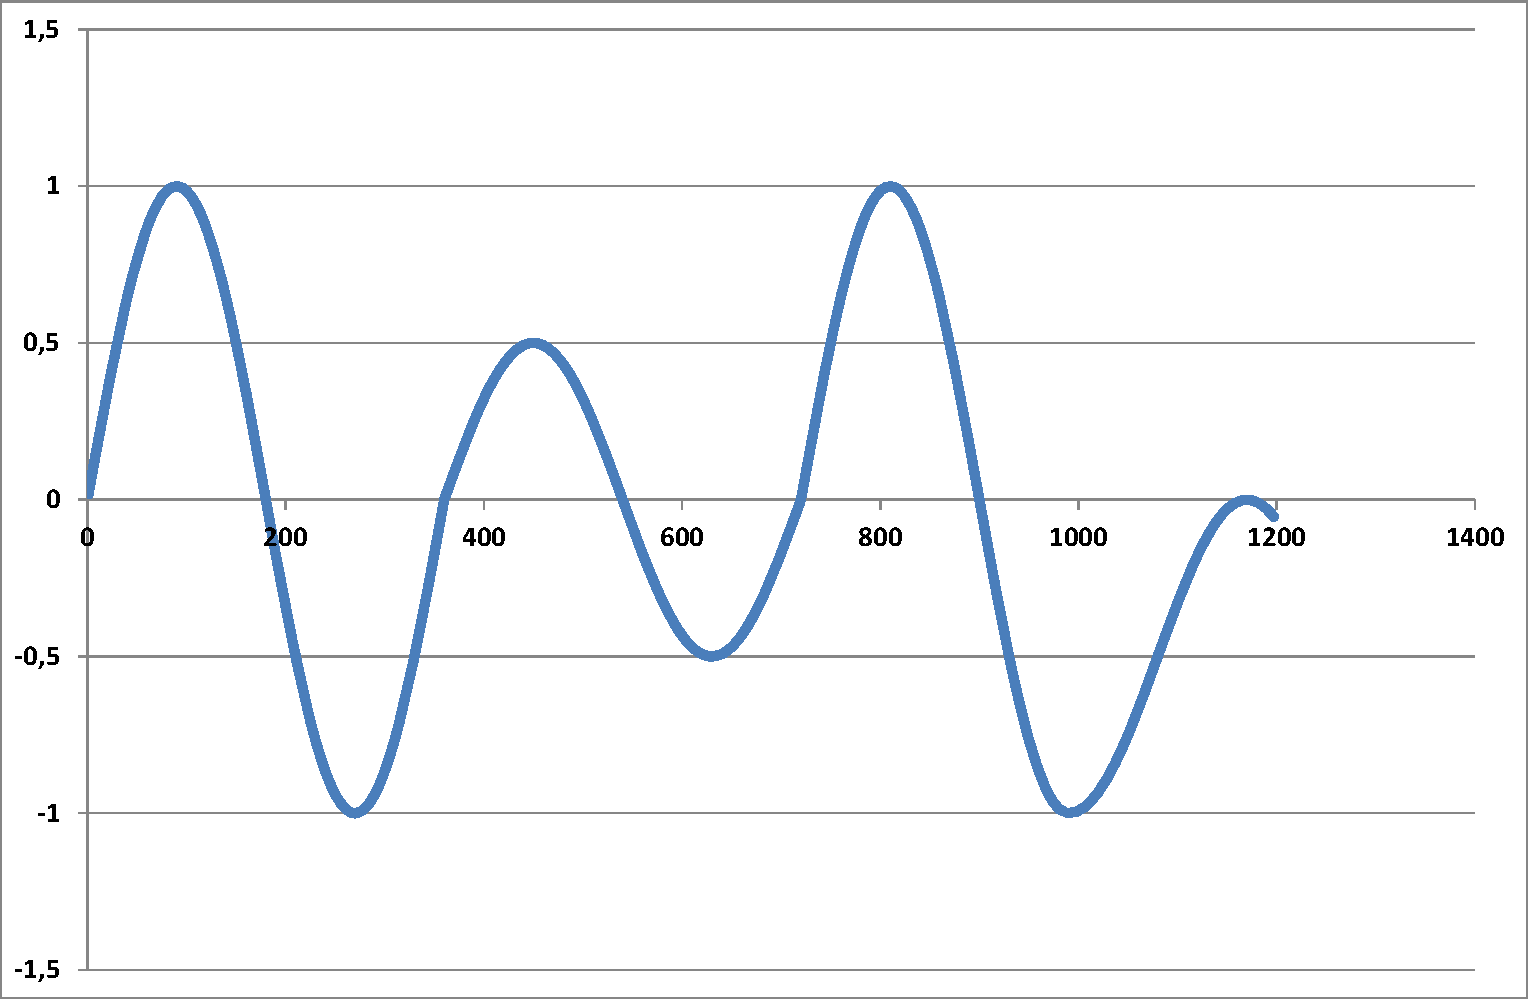
\includegraphics[width=0.28\linewidth]{img/analogique} & 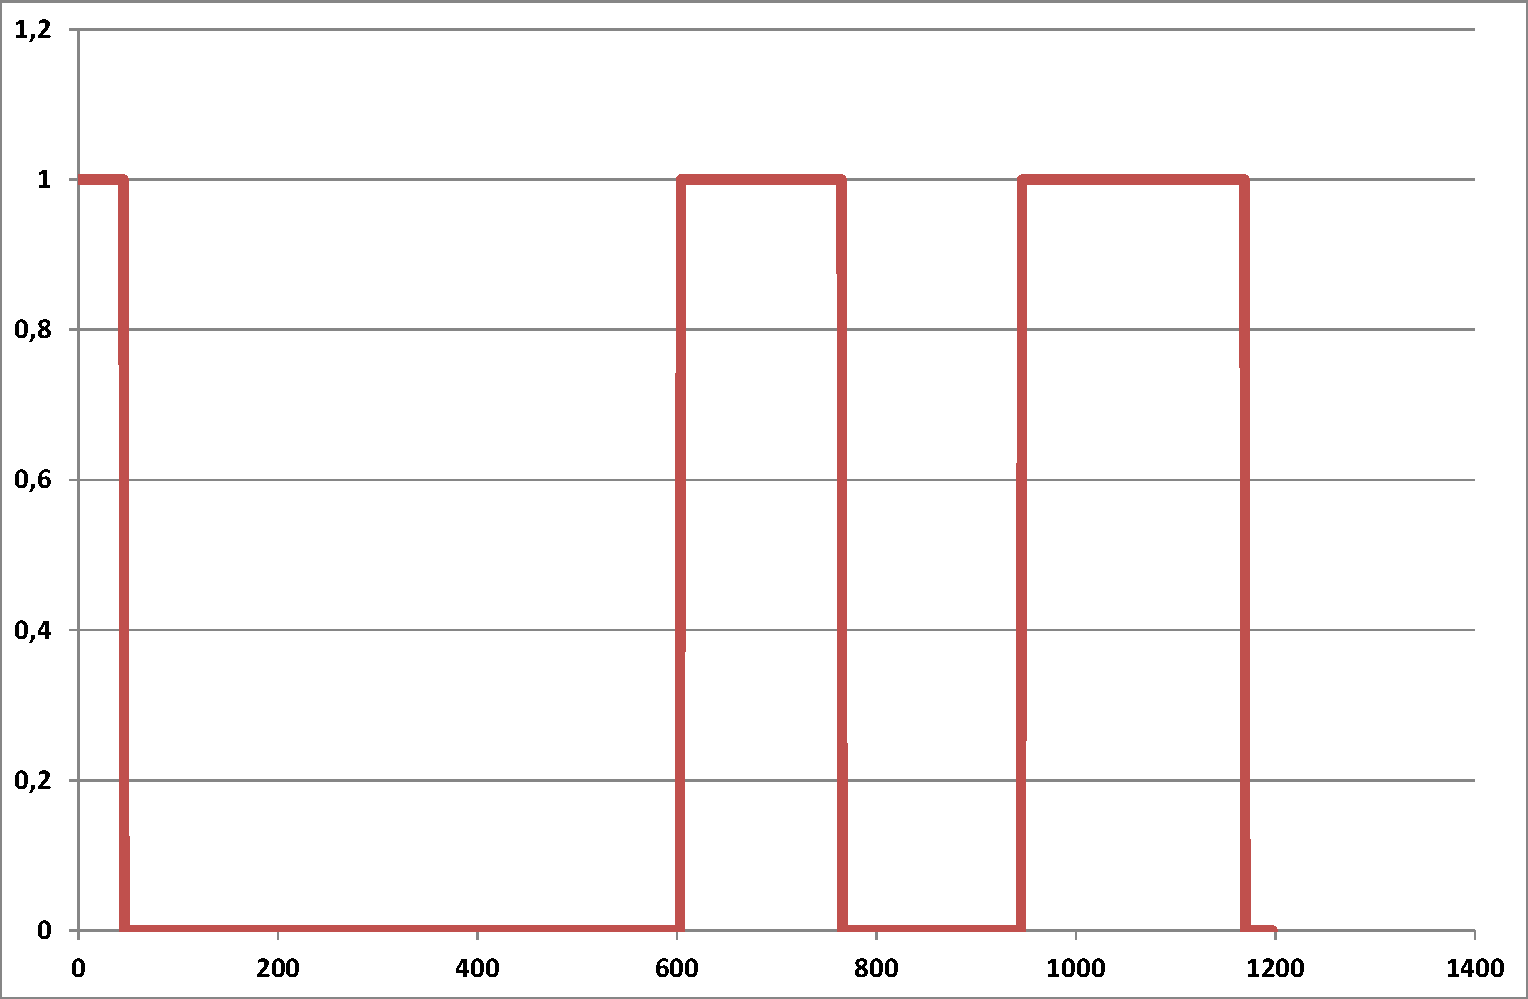
\includegraphics[width=0.28\linewidth]{img/logique} &
	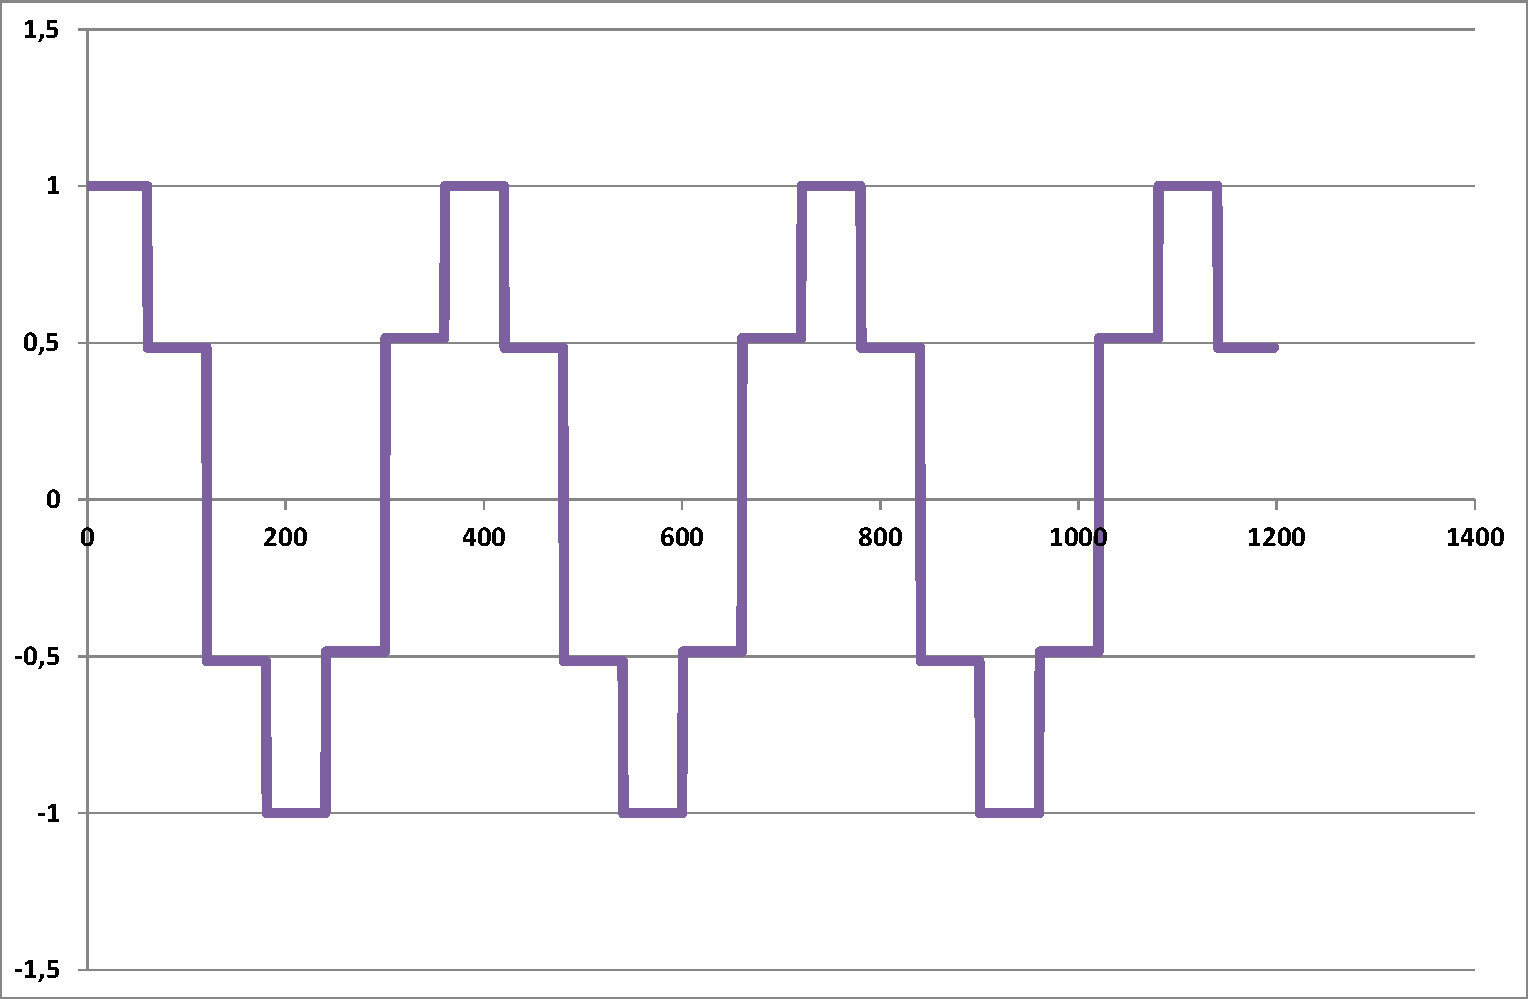
\includegraphics[width=0.28\linewidth]{img/numerique} \\
	\ifdef{\public}{Analogique}{..........} & \ifdef{\public}{Logique}{..........} & \ifdef{\public}{Numérique}{..........}
	\end{tabular}
\end{center}

}}

{\frame{
\frametitle{Acquérir}

La fonction \textbf{Acquérir} consiste à prélever les informations venant du système ou de l'utilisateur qui servent à faire évoluer l'état du système.

\vfill

\begin{tabular}{c c}
\begin{minipage}{0.47\linewidth}
L'\textbf{utilisateur} envoie ses \textbf{ordres} au système par l'intermédiaire d'un \textbf{pupitre de commande}.\end{minipage} &
\begin{minipage}{0.47\linewidth}
Les informations sont \textbf{prélevées} sur le système par l'intermédiaire de \textbf{capteurs}. \end{minipage} \\ \\
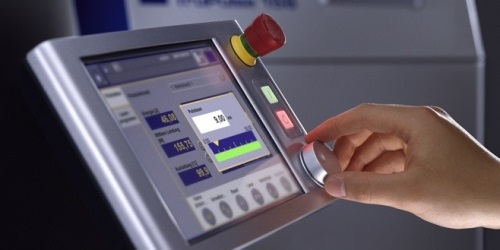
\includegraphics[width=0.47\linewidth]{img/pupitre} & 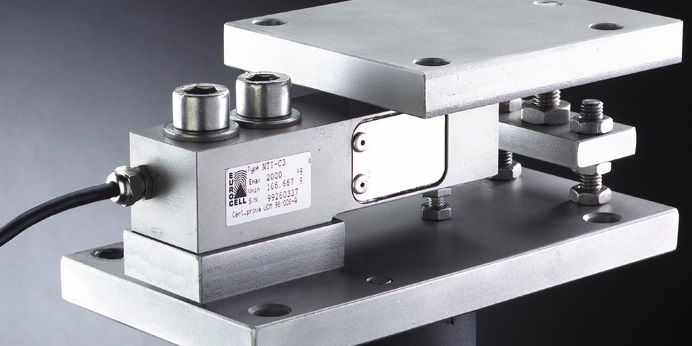
\includegraphics[width=0.47\linewidth]{img/capteur_indus}
\end{tabular}

L'étude des pupitres n'étant pas un de nos objectifs, nous allons nous découvrir l'éventail des capteurs mis à notre disposition.

}}

{\frame{
\frametitle{Les capteurs}

Un capteur \textbf{prélève} une information sur le comportement de la \textbf{partie opérative} et la \textbf{transforme} en une \textbf{information} exploitable par la \textbf{partie commande}. 

\vfill

Pour pouvoir être traitée, cette information sera \textbf{portée} par un support physique (énergie), on parlera alors de \textbf{signal}. Les signaux sont généralement de nature \textbf{électrique} ou \textbf{pneumatique}.

\vfill

Les capteurs peuvent être caractérisés selon deux critères:
\begin{itemize}
 \item la \textbf{grandeur mesurée}: capteurs de position, de température, de vitesse, de force, de pression, etc...
 \item le caractère de l'\textbf{information} délivrée: capteurs logiques, analogiques ou numériques.
 \item l'\textbf{interaction} avec l'objet à détecter: capteurs de contact et de proximité.
\end{itemize} 

}}


{\frame{
\frametitle{Les capteurs}
Principales caractéristiques des capteurs:
\begin{itemize}
 \item L'\textbf{étendue de la mesure:} différence entre le plus petit signal détecté et le plus grand perceptible sans risque de destruction pour le capteur,
 \item La \textbf{sensibilité:} plus petite variation d'une grandeur physique que peut détecter un capteur,
 \item La \textbf{rapidité:} temps de réaction d'un capteur entre la variation de la grandeur physique qu'il mesure et l'instant où l'information est prise en compte par la partie commande,
 \item La \textbf{précision:} capabilité de répétabilité d'une information position, d'une vitesse,...
\end{itemize}

\begin{center}
	\begin{tabular}{c c c}
	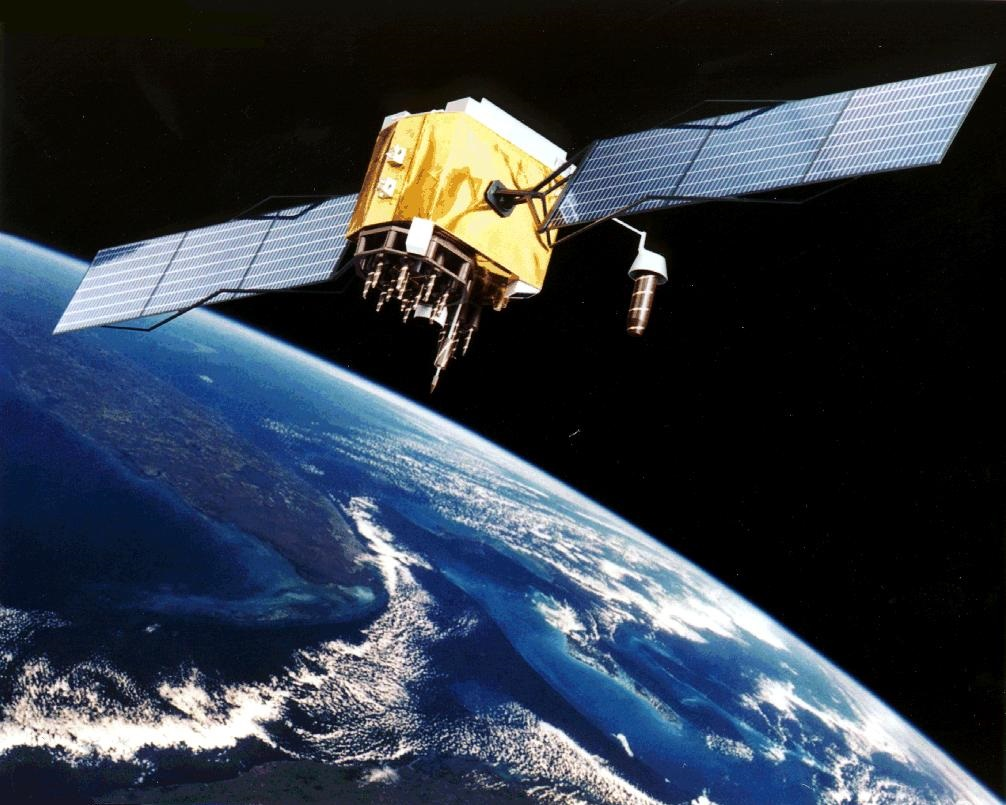
\includegraphics[width=0.28\linewidth]{img/satellite} & 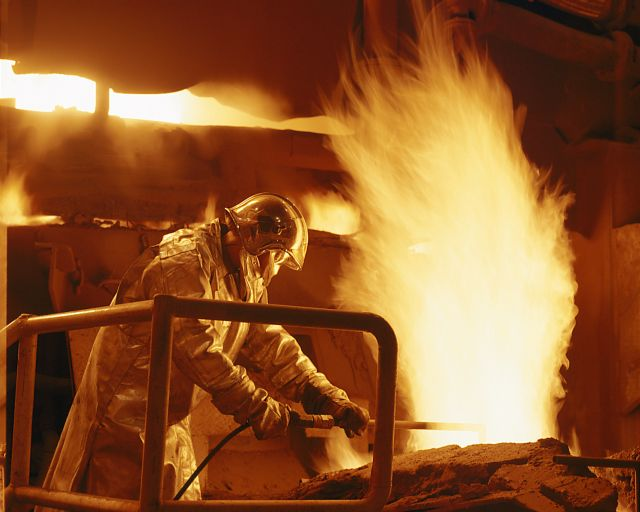
\includegraphics[width=0.28\linewidth]{img/forge} &
	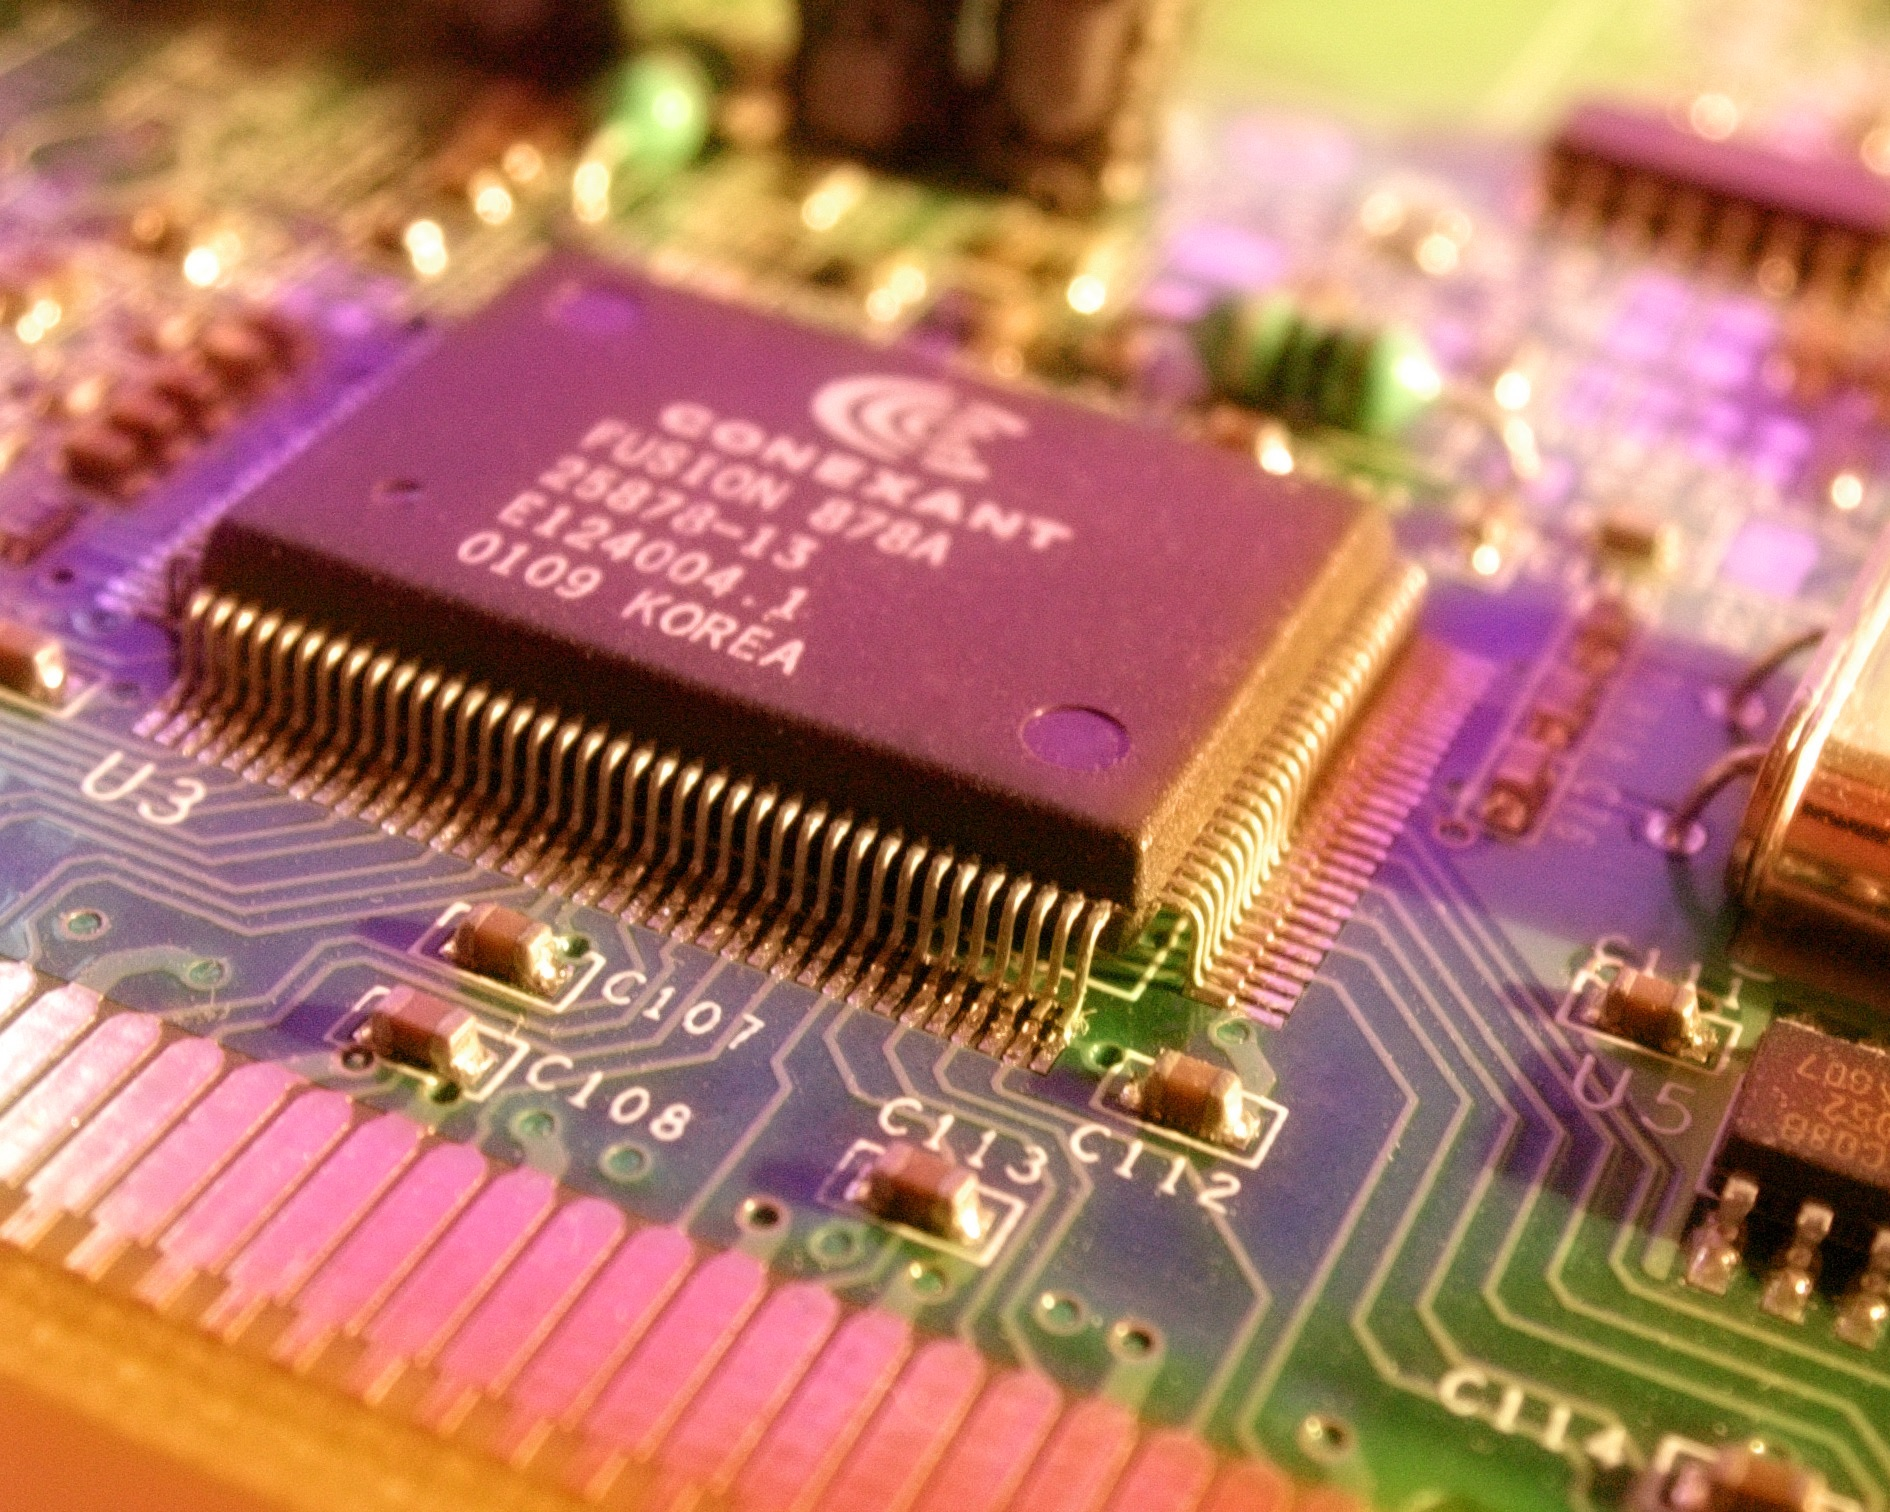
\includegraphics[width=0.28\linewidth]{img/electronique}
	\end{tabular}
\end{center}

}}

{\frame{
\frametitle{Les capteurs}

\begin{tabular}{|c|c|c|}
\hline
\begin{minipage}{0.3\linewidth} \textbf{Capteurs à seuil de pression pneumatique} \end{minipage} & \begin{minipage}{0.4 \linewidth} Ce sont des capteurs fin de course qui se montent directement sur les vérins. \end{minipage} & \begin{minipage}{0.2 \linewidth} \vspace{5pt} \centering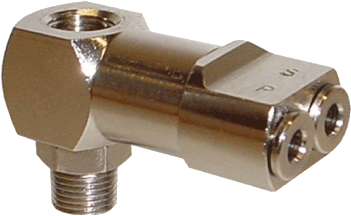
\includegraphics[width=0.8\linewidth]{img/capteur1} \vspace{5pt} \end{minipage} \\
\hline
\begin{minipage}{0.3\linewidth} \textbf{Capteur capacitif} \end{minipage} & \begin{minipage}{0.4 \linewidth}Les capteurs capacitifs sont des capteurs de proximité qui permettent de détecter des objets métalliques ou isolants. \end{minipage} & \begin{minipage}{0.2 \linewidth} \vspace{5pt} \centering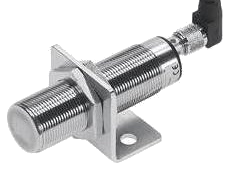
\includegraphics[width=0.8\linewidth]{img/capteur2} \vspace{5pt} \end{minipage} \\
\hline
\begin{minipage}{0.3\linewidth} \textbf{Capteur inductif} \end{minipage} & \begin{minipage}{0.4 \linewidth} Les capteurs inductifs produisent à l'extrémité de leur tête de détection un champ magnétique oscillant perturbé en présence d'un objet. \end{minipage} & \begin{minipage}{0.2 \linewidth} \vspace{5pt} \centering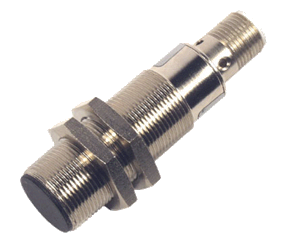
\includegraphics[width=0.8\linewidth]{img/capteur3} \vspace{5pt} \end{minipage} \\
\hline
\end{tabular}
}}

{\frame{
\frametitle{Les capteurs}

\begin{tabular}{|c|c|c|}
\hline
\begin{minipage}{0.3\linewidth} \textbf{Capteurs à contact} \end{minipage} & \begin{minipage}{0.4 \linewidth} Les capteurs de contact peuvent être équipé d'un galet, d'une tige souple, d'une bille. Capteurs tout ou rien (électrique ou pneumatique). \end{minipage} & \begin{minipage}{0.2 \linewidth} \vspace{5pt} \centering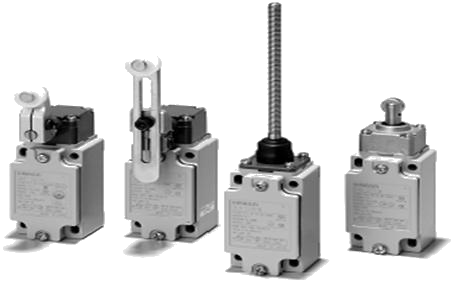
\includegraphics[width=\linewidth]{img/capteur4} \vspace{5pt} \end{minipage} \\
\hline
\begin{minipage}{0.3\linewidth} \textbf{Capteur ILS} \end{minipage} & \begin{minipage}{0.4 \linewidth} Un capteur ILS est composé d'une lame souple sensible à la présence d'un champ magnétique mobile.
\end{minipage} & \begin{minipage}{0.2 \linewidth} \vspace{5pt} \centering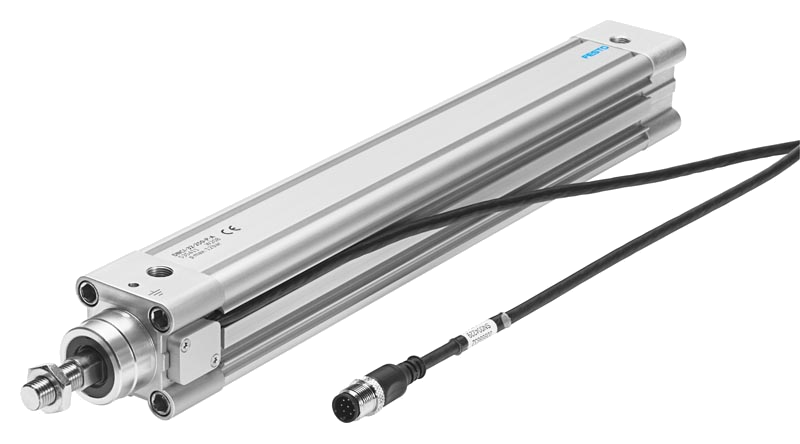
\includegraphics[width=0.8\linewidth]{img/capteur5} \vspace{5pt} \end{minipage} \\
\hline
\begin{minipage}{0.3\linewidth} \textbf{Capteur optique} \end{minipage} & \begin{minipage}{0.4 \linewidth} Un capteur photoélectrique est un capteur de proximité. Il se compose d'un émetteur de lumière associé à un récepteur. \end{minipage} & \begin{minipage}{0.2 \linewidth} \vspace{5pt} \centering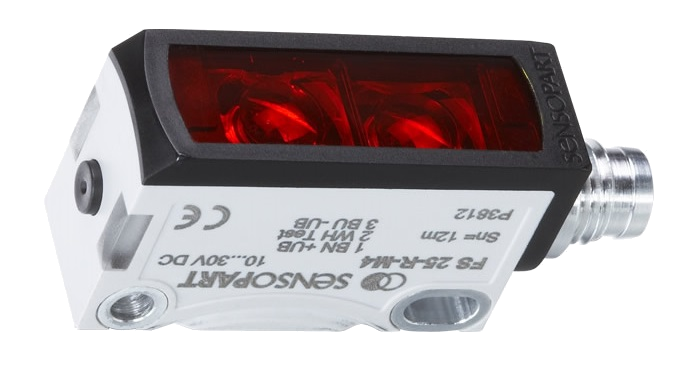
\includegraphics[width=0.8\linewidth]{img/capteur6} \vspace{5pt} \end{minipage} \\
\hline
\end{tabular}
}}


{\frame{
\frametitle{Les capteurs}

\begin{tabular}{|c|c|c|}
\hline
\begin{minipage}{0.3\linewidth} \textbf{Codeur rotatif incrémental} \end{minipage} & \begin{minipage}{0.4 \linewidth} Les codeurs rotatifs sont des capteurs de position angulaire. Le disque du codeur est solidaire de l'arbre tournant du système à contrôler. \end{minipage} & \begin{minipage}{0.2 \linewidth} \vspace{5pt} \centering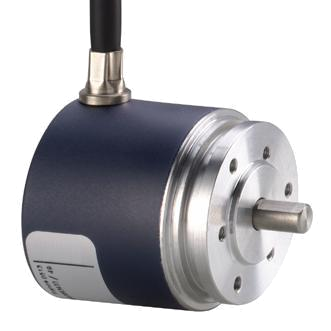
\includegraphics[width=0.6\linewidth]{img/capteur7} \vspace{5pt} \end{minipage} \\
\hline
\begin{minipage}{0.3\linewidth} \textbf{Codeur rotatif absolu} \end{minipage} & \begin{minipage}{0.4 \linewidth} Dans le cas de ce capteur, la piste est codée afin de déterminer la position angulaire du codeur. \end{minipage} & \begin{minipage}{0.2 \linewidth} \vspace{5pt} \centering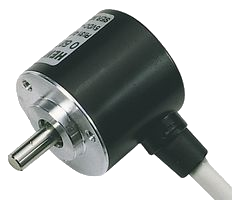
\includegraphics[width=0.6\linewidth]{img/capteur8} \vspace{5pt} \end{minipage} \\
\hline
\end{tabular}

\begin{minipage}{0.6\linewidth} Le code binaire réfléchi (présenté plus tard) a été mis en place afin d'être utilisé sur ces codeurs. \end{minipage} \hfill \begin{minipage}{0.3 \linewidth} \vspace{5pt} \centering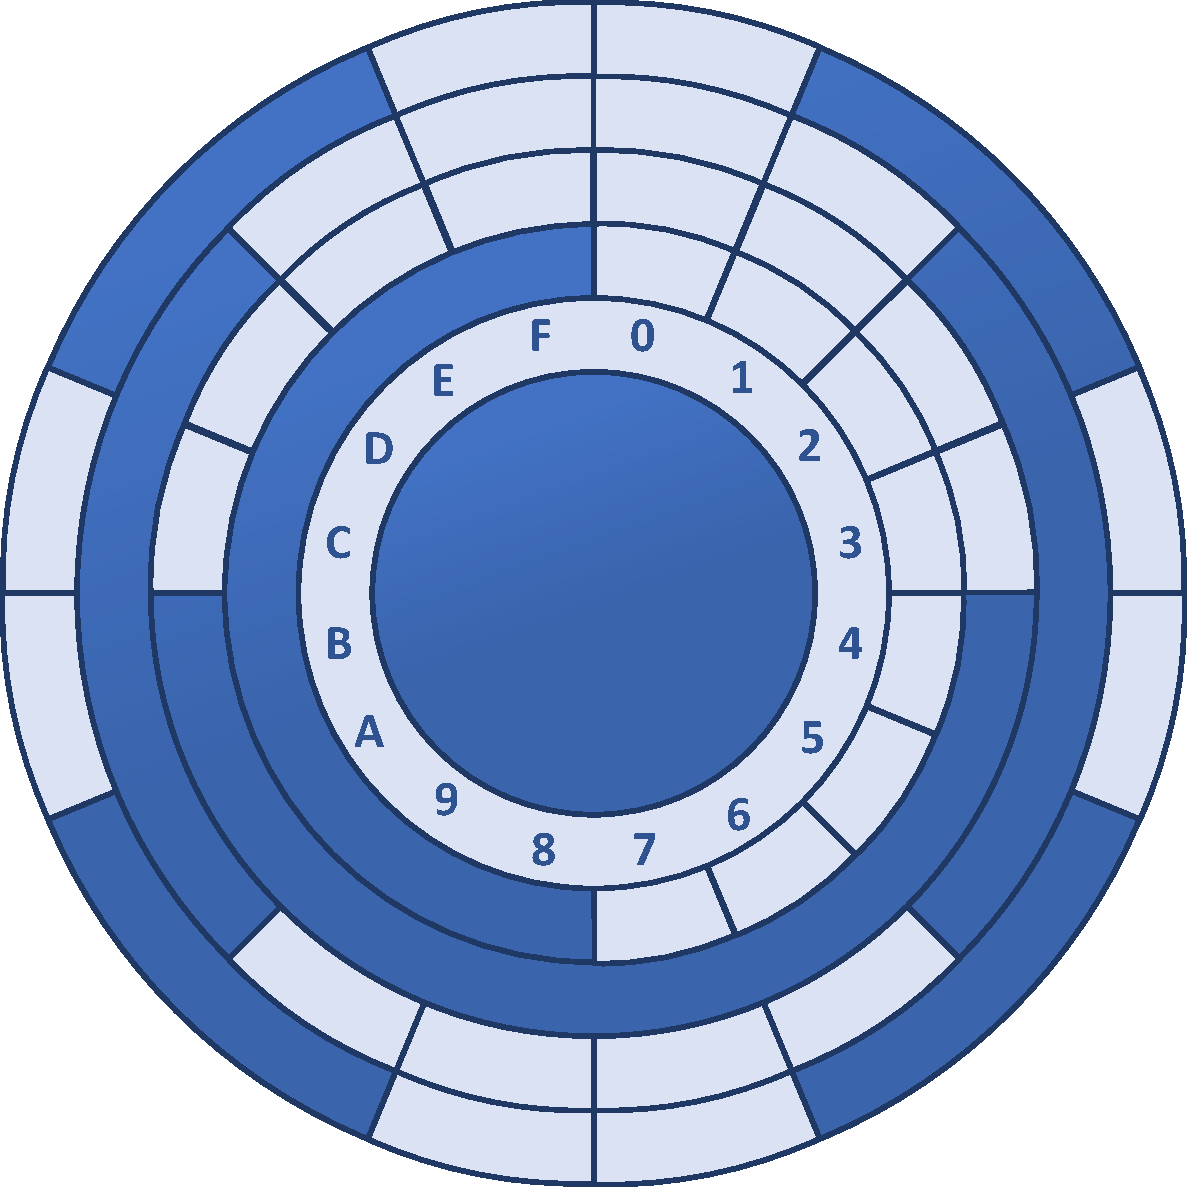
\includegraphics[width=.8\linewidth]{img/codeur_absolu} \vspace{5pt} \end{minipage}
}}

{\frame{
\frametitle{Les capteurs}

\begin{tabular}{|c|c|c|}
\hline
\begin{minipage}{0.3\linewidth} \textbf{Jauge de contrainte} \end{minipage} & \begin{minipage}{0.4 \linewidth} La résistance ohmique de la jauge varie en fonction des déformations générées par la contrainte. \end{minipage} & \begin{minipage}{0.2 \linewidth} \vspace{5pt} \centering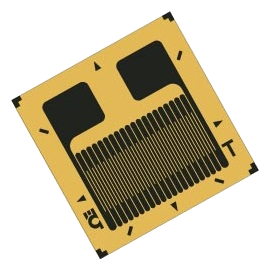
\includegraphics[width=0.8\linewidth]{img/capteur9} \vspace{5pt} \end{minipage} \\
\hline
\begin{minipage}{0.3\linewidth} \textbf{Thermocouples} \end{minipage} & \begin{minipage}{0.4 \linewidth} La différence de température entre les deux jonctions du capteur fait varier sa résistance ohmique. \end{minipage} & \begin{minipage}{0.2 \linewidth} \vspace{5pt} \centering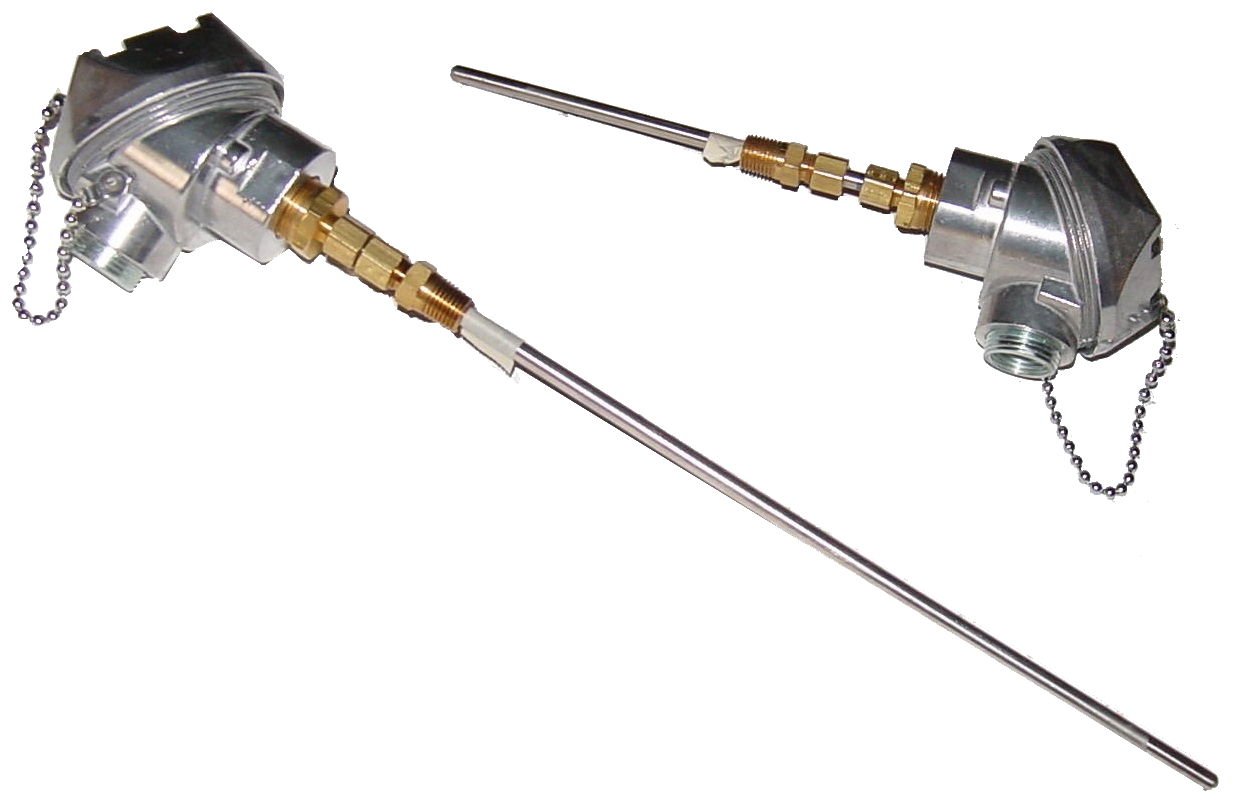
\includegraphics[width=0.8\linewidth]{img/capteur10} \vspace{5pt} \end{minipage} \\
\hline
\begin{minipage}{0.3\linewidth} \textbf{Génératrice tachymétrique} \end{minipage} & \begin{minipage}{0.4 \linewidth} Un capteur tachymétrique agit comme un générateur analogique, la tension à sa sortie est proportionnelle à la vitesse de rotation. \end{minipage} & \begin{minipage}{0.2 \linewidth} \vspace{5pt} \centering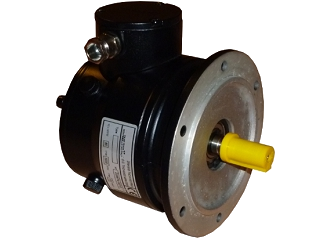
\includegraphics[width=0.8\linewidth]{img/capteur11} \vspace{5pt} \end{minipage} \\
\hline
\end{tabular}
}}

{\frame{
\frametitle{Le choix d'un capteur}

Le choix d'un capteur se fait alors en prenant en compte les critères suivants:
\begin{itemize}
 \item le type événement à détecter,
 \item la nature de événement,
 \item La grandeur de l'événement,
 \item l'environnement de l'événement.
\end{itemize}


En fonction de ces paramètres on pourra effectuer un ou plusieurs choix pour un type de détection. D'autres critères permettent d'optimiser ce choix:
\begin{itemize}
 \item ses performances,
 \item son encombrement,
 \item sa fiabilité (MTBF)
 \item la nature du signal délivré par le capteur (électrique, pneumatique)
 \item son prix...
\end{itemize}
}}

{\frame{
\frametitle{Traiter}

La fonction \textbf{Traiter} consiste à suivre l'\textbf{algorithme} de gestion du comportement du système en fonction des informations issues de l'étape précédente.

\vfill

La \textbf{Partie Commande} d'un automatisme est le centre de décision. Elle donne des ordres à la partie opérative et reçoit ses comptes rendus.

\vfill

\begin{tabular}{|c|c|c|}
\hline
\begin{minipage}{0.3\linewidth} \textbf{Automate Programmable Industriel} \end{minipage} & \begin{minipage}{0.4 \linewidth} Dispositif électronique programmable pour la commande de processus industriels par un traitement séquentiel.  \end{minipage} & \begin{minipage}{0.2 \linewidth} \vspace{5pt} \centering\includegraphics[width=0.7\linewidth]{img/traiter1} \vspace{5pt} \end{minipage} \\
\hline
\begin{minipage}{0.3\linewidth} \textbf{Micro-contrôleur} \end{minipage} & \begin{minipage}{0.4 \linewidth} Circuit qui rassemble des éléments d'un ordinateur : processeur, mémoires, interfaces d'entrées-sorties,... \end{minipage} & \begin{minipage}{0.2 \linewidth} \vspace{5pt} \centering\includegraphics[width=0.7\linewidth]{img/traiter2} \vspace{5pt} \end{minipage} \\
\hline
\begin{minipage}{0.3\linewidth} \textbf{Micro-processeur} \end{minipage} & \begin{minipage}{0.4 \linewidth} Processeur dont les composants ont été miniaturisés pour être regroupés dans un unique circuit intégré.  \end{minipage} & \begin{minipage}{0.2 \linewidth} \vspace{5pt} \centering\includegraphics[width=0.7\linewidth]{img/traiter3} \vspace{5pt} \end{minipage} \\
\hline
\end{tabular}
}}

{\frame{
\frametitle{Communiquer}

La fonction \textbf{Communiquer} consiste à transmettre les informations/ordres au parties concernées.

\vfill

La \textbf{Partie Commande} d'un automatisme est le centre de décision. Elle donne des ordres à la partie opérative et reçoit ses comptes rendus.

\vfill

\begin{tabular}{c c c}
\begin{minipage}{0.3\linewidth} Les distributeurs reçoivent les ordres via des câbles. \end{minipage} & 
\multicolumn{2}{c}{\begin{minipage}{0.6\linewidth} L'\textbf{utilisateur} reçois des \textbf{informations} du système par l'intermédiaire d'un \textbf{pupitre de commande} ou de voyants \end{minipage} } \\ \\
\includegraphics[width=0.3\linewidth]{img/communiquer1} & \includegraphics[width=0.3\linewidth]{img/pupitre}& \includegraphics[width=0.3\linewidth]{img/communiquer2}
\end{tabular}

}}

\end{document}

